% !TEX program = xelatex
\documentclass[10pt,aspectratio=169,xcolor={dvipsnames}]{beamer}
\usetheme[progressbar=frametitle,block=fill]{metropolis}
\metroset{sectionpage=none}
\setbeamercolor{background canvas}{bg=white}

% Duke palette from the supplied Slides_template.
\definecolor{DukeNavyBlue}{HTML}{012169}
\definecolor{DukeRoyalBlue}{HTML}{00539B}
\definecolor{SoftBlue}{HTML}{EAF3FF}
\definecolor{SoftGray}{HTML}{F5F7FA}
\definecolor{PaperGray}{HTML}{4E5A66}
\definecolor{AlertRed}{HTML}{B31B1B}
\definecolor{GoodGreen}{HTML}{2E7D32}
\definecolor{WarnOrange}{HTML}{955D00}
\definecolor{AtlasBlue}{HTML}{1238E8}
\definecolor{TeamPurple}{HTML}{8C52FF}
\definecolor{TeamGreen}{HTML}{00A85A}
\definecolor{TeamGold}{HTML}{FFD95A}
\definecolor{TeamInk}{HTML}{17324D}
\definecolor{TeamMist}{HTML}{F8F6FF}
\definecolor{CalloutFill}{HTML}{FFF1E8}
\definecolor{CalloutBorder}{HTML}{DFA886}
\usepackage{tikz}
\usepackage{tikzpagenodes} % provides the `current page` node for page-relative TikZ placement

\setbeamercolor{progress bar}{fg=DukeRoyalBlue,bg=gray!20}
\setbeamercolor{title separator}{fg=DukeRoyalBlue}
\setbeamercolor{frametitle}{bg=DukeRoyalBlue,fg=white}
\setbeamercolor{alerted text}{fg=DukeRoyalBlue}
\setbeamercolor{itemize item}{fg=DukeRoyalBlue}
\setbeamercolor{itemize subitem}{fg=DukeRoyalBlue}
\setbeamercolor{block title}{fg=white,bg=DukeRoyalBlue}
\setbeamercolor{block body}{fg=black,bg=SoftBlue}
\setbeamercolor{project distinction}{fg=white,bg=DukeRoyalBlue}
\setbeamercolor{paperfooter}{fg=PaperGray,bg=SoftGray}
\setbeamersize{text margin left=0.035\paperwidth,text margin right=0.035\paperwidth}
\setbeamertemplate{navigation symbols}{}
\setbeamerfont{title}{size=\fontsize{26}{30}\selectfont,series=\bfseries}
\setbeamerfont{subtitle}{size=\fontsize{13}{16}\selectfont}
\setbeamerfont{author}{size=\fontsize{10.5}{13}\selectfont}
\setbeamerfont{date}{size=\fontsize{9}{11}\selectfont}
\setbeamerfont{institute}{size=\scriptsize}
\setbeamerfont{frametitle}{size=\fontsize{15}{18}\selectfont,series=\bfseries}

\usepackage{fontspec}
\IfFontExistsTF{Avenir Next}{\setsansfont{Avenir Next}}{%
  \IfFontExistsTF{TeX Gyre Heros}{\setsansfont{TeX Gyre Heros}}{\setsansfont{Latin Modern Sans}}}
\IfFontExistsTF{Menlo}{\setmonofont{Menlo}}{%
  \IfFontExistsTF{TeX Gyre Cursor}{\setmonofont{TeX Gyre Cursor}}{\setmonofont{Latin Modern Mono}}}
\usepackage{booktabs}
\usepackage{tikz}
\usepackage{amsmath,amssymb,amsfonts}
\usepackage{graphicx}
\usepackage{textcomp}
\usepackage{multirow}
\usepackage{colortbl}
\usepackage{array}
\usepackage{tabularx}
\usepackage[numbers,sort&compress]{natbib}
\usepackage{multicol}
\usepackage{hyperref}
\usepackage{pifont}
\usetikzlibrary{positioning,calc,shapes.geometric}
\graphicspath{{figures/}{figures/technical_clip_art/assets/}{./}}

% A fixed-height title bar protects ascenders from the page edge.  The icon is
% positioned independently, so it can never push a long title outside the page.
\setbeamertemplate{frametitle}{%
  \nointerlineskip%
  \begin{beamercolorbox}[wd=\paperwidth,ht=0.72cm,dp=0.18cm,
      leftskip=0.52cm,rightskip=1.28cm]{frametitle}%
    \usebeamerfont{frametitle}\strut\insertframetitle\strut\par
  \end{beamercolorbox}%
  \usebeamertemplate*{progress bar in head/foot}%
}

\newcommand{\icontitle}[2]{%
  \texorpdfstring{#1\hfill\llap{%
    \raisebox{-0.13cm}[0pt][0pt]{%
      \begin{tikzpicture}[baseline=(icon.base)]
        \node[fill=white,rounded corners=1.5pt,inner sep=1.4pt,
          minimum width=0.61cm,minimum height=0.61cm] (icon)
          {\includegraphics[height=0.48cm]{#2}};
      \end{tikzpicture}}}}{#1}%
}

\newcommand{\titlepageclip}[1]{%
  \begin{tikzpicture}[remember picture,overlay]
    \node[anchor=south east,inner sep=0pt]
      at ([xshift=-0.62cm,yshift=0.52cm]current page.south east)
      {\includegraphics[width=2.85cm]{#1}};
  \end{tikzpicture}%
}

\hypersetup{
  colorlinks=true,
  linkcolor=DukeRoyalBlue,
  citecolor=DukeRoyalBlue,
  urlcolor=DukeRoyalBlue
}

\newcommand{\claimbox}[1]{%
  \begin{beamercolorbox}[wd=\linewidth,sep=4pt,rounded=true]{block body}
    #1
  \end{beamercolorbox}
}
\newcommand{\sourcefoot}[1]{%
  \begin{tikzpicture}[remember picture,overlay]
    \node[anchor=south,yshift=0.13cm,inner xsep=2pt,inner ysep=1pt,
      fill=white,text width=0.87\paperwidth,align=left,
      font=\fontsize{6.6}{7.4}\selectfont\itshape,text=PaperGray]
      at (current page.south) {#1};
  \end{tikzpicture}%
}
\newcommand{\smalllead}[1]{%
  {\large\bfseries\color{DukeNavyBlue}#1}
}
\newcommand{\metric}[2]{%
  \begin{beamercolorbox}[wd=0.95\linewidth,sep=4pt,rounded=true,center]{block body}
    {\Large\textbf{#1}}\\[-1pt]
    {\scriptsize #2}
  \end{beamercolorbox}
}

\newcommand{\profilephoto}[4]{%
  \begin{tikzpicture}[baseline=(current bounding box.center)]
    \path[use as bounding box] (-#2,-#2) rectangle (#2,#2);
    \begin{scope}
      \clip (0,0) circle (#2);
      \node[yshift=#4] at (0,0) {\includegraphics[width=#3]{#1}};
    \end{scope}
    \draw[TeamPurple!70,line width=1.1pt] (0,0) circle (#2);
  \end{tikzpicture}%
}
\newcommand{\profilelabel}[1]{%
  {\fontsize{10.5}{12.5}\selectfont\bfseries\color{TeamGreen}#1}\par
  \vspace{0.10cm}%
}
\newcommand{\stacanvas}{%
  \begin{tikzpicture}[remember picture,overlay]
    \shade[left color=TeamPurple,right color=TeamGreen]
      (current page.south west) rectangle (current page.north east);
    \fill[white]
      ([xshift=0.18cm,yshift=0.18cm]current page.south west)
      rectangle
      ([xshift=-0.18cm,yshift=-0.18cm]current page.north east);
  \end{tikzpicture}%
}
\newcommand{\staheading}[3]{%
  \begin{tikzpicture}[remember picture,overlay]
    \node[anchor=north west,text=TeamGreen,
      font=\fontsize{15.5}{17.5}\selectfont\bfseries]
      at ([xshift=0.58cm,yshift=-0.30cm]current page.north west) {#1};
    \node[anchor=north west,text=TeamInk,
      font=\fontsize{8.2}{9.8}\selectfont\bfseries]
      at ([xshift=0.58cm,yshift=-0.82cm]current page.north west) {#2};
    \node[anchor=north east,inner sep=0pt]
      at ([xshift=-0.58cm,yshift=-0.25cm]current page.north east)
      {\includegraphics[height=0.78cm]{#3}};
    \shade[left color=TeamPurple,right color=TeamGreen]
      ([xshift=0.58cm,yshift=-1.25cm]current page.north west)
      rectangle
      ([xshift=-0.58cm,yshift=-1.20cm]current page.north east);
  \end{tikzpicture}%
}
\newcommand{\staoverviewclip}[1]{%
  \begin{tikzpicture}[remember picture,overlay]
    \node[anchor=north east,inner sep=0pt]
      at ([xshift=-0.56cm,yshift=-0.38cm]current page.north east)
      {\includegraphics[height=1.10cm]{#1}};
  \end{tikzpicture}%
}

\setbeamertemplate{bibliography item}{\insertbiblabel}
\makeatletter
\newcommand{\compactbibliography}[1]{%
  \begingroup
  \renewcommand{\section}{\@ifstar{\@gobble}{\@gobble}}%
  \bibliography{#1}%
  \endgroup
}
\makeatother

\title{ContextLens}
\subtitle{An Evidence-Grounded Agent for Verifiable Historical Address Investigation}
\date{September 2026}

\author[ContextLens]{%
  Shilin Ou$^{+}$ \and
  Sean Wan$^{+}$ \and
  Yutian Wang \and
  Polina Postnikova \and
  Luyao Zhang$^{*}$
}

\institute{%
  Duke Kunshan University (DKU)\\[1pt]
  \textcolor{DukeRoyalBlue}{Submitted to AAAI-27 Demonstrations. Do not circulate or distribute.}
}

\begin{document}
\bibliographystyle{IEEEtran}

\begin{frame}[plain,t]
  \raggedright
  \vspace*{0.25cm}

  {\usebeamerfont{title}\usebeamercolor[fg]{title}\inserttitle
    \titlepageclip{context-lens-hero.pdf}\par}
  \vspace{0.18cm}
  {\usebeamerfont{subtitle}\usebeamercolor[fg]{subtitle}\insertsubtitle\par}
  \vspace{0.18cm}
  {\usebeamercolor[fg]{title separator}\rule{\linewidth}{0.5pt}\par}
  \vspace{0.32cm}

  {\usebeamerfont{author}\usebeamercolor[fg]{author}
    Shilin Ou$^{+}$\quad
    Sean Wan$^{+}$\quad
    Yutian Wang\quad
    Polina Postnikova\quad
    Luyao Zhang$^{*}$\par}
  \vspace{0.08cm}
  {\usebeamerfont{date}\insertdate\par}
  \vspace{0.12cm}
  {\usebeamerfont{institute}\insertinstitute\par}

  % One compact author-note line stays safely inside the 16:9 frame.
  \vspace{0.20cm}
  {\fontsize{7.5}{9}\selectfont\color{PaperGray}
    \rule{0.32\paperwidth}{0.3pt}\par
    \vspace{2pt}
    \textsuperscript{+}\,Joint first authors.
    \qquad
    \textsuperscript{*}\,Corresponding author:
    \href{mailto:lz183@duke.edu}{lz183@duke.edu}.\par}
  \vfill
\end{frame}

\section{Motivation}

\begin{frame}[t]{\icontitle{Why historical addresses are difficult to verify}{archive-place.pdf}}
\small
\begin{columns}[T,onlytextwidth]
\column{0.46\textwidth}
\smalllead{Dated place names change meaning over time}

\vspace{0.25em}
\begin{itemize}
  \item Street names change across time.
  \item Numbers and landmarks remain ambiguous.
  \item Archival coverage is uneven.
  \item Fluent answers exceed available evidence.
\end{itemize}

\vspace{0.10em}
\claimbox{\textbf{Research Question:} How can an agent resolve a dated place before retrieval and keep each claim inspectable?}

\column{0.50\textwidth}
\centering
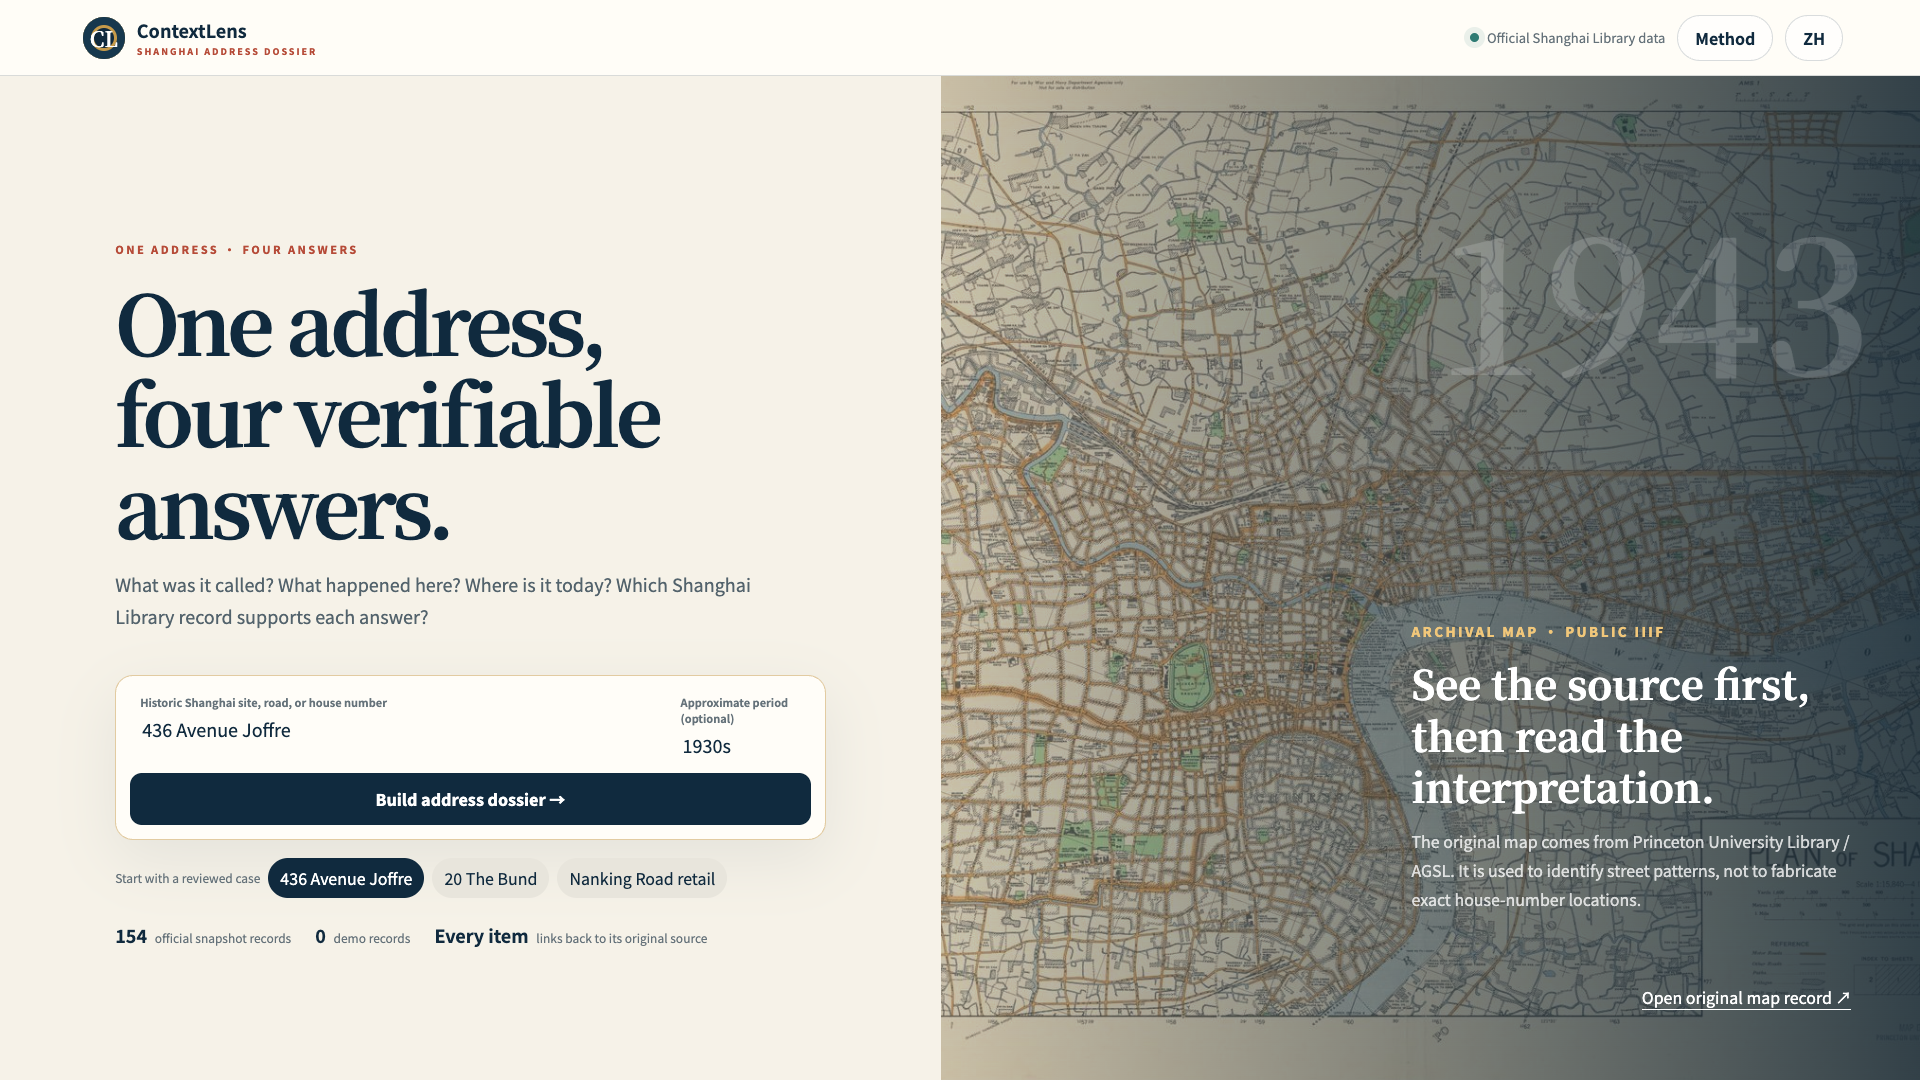
\includegraphics[width=\linewidth]{ui_home_en.png}

\vspace{0.35em}
The interface starts from one address and asks four source-backed questions.
\end{columns}
\sourcefoot{Motivation: \citep{southall2011gazetteers}. Current interface capture, 10 September 2026.}
\note{Historical addresses change over time. The task requires temporal identity resolution before any historical claim is made.}
\end{frame}

\begin{frame}[t]{\icontitle{Place identity resolution before retrieval}{identity-resolution.pdf}}
\begin{columns}[T,onlytextwidth]
\column{0.52\textwidth}
\small
\smalllead{Core design}

\vspace{0.20em}
\normalsize A dated address becomes a typed, replayable investigation.

\vspace{0.42em}
\textcolor{DukeRoyalBlue}{\textbf{01}}\quad\textbf{Temporal place resolution}\\[-1pt]
{\small Dated aliases and competing candidates remain visible.}

\vspace{0.42em}
\textcolor{DukeRoyalBlue}{\textbf{02}}\quad\textbf{Relation and claim gates}\\[-1pt]
{\small Only place- and time-compatible evidence can support a claim.}

\vspace{0.42em}
\textcolor{DukeRoyalBlue}{\textbf{03}}\quad\textbf{Source Passports}\\[-1pt]
{\small Provider, dataset, period, evidence ID, normalization state, and original URI travel with each record.}

\column{0.44\textwidth}
\centering
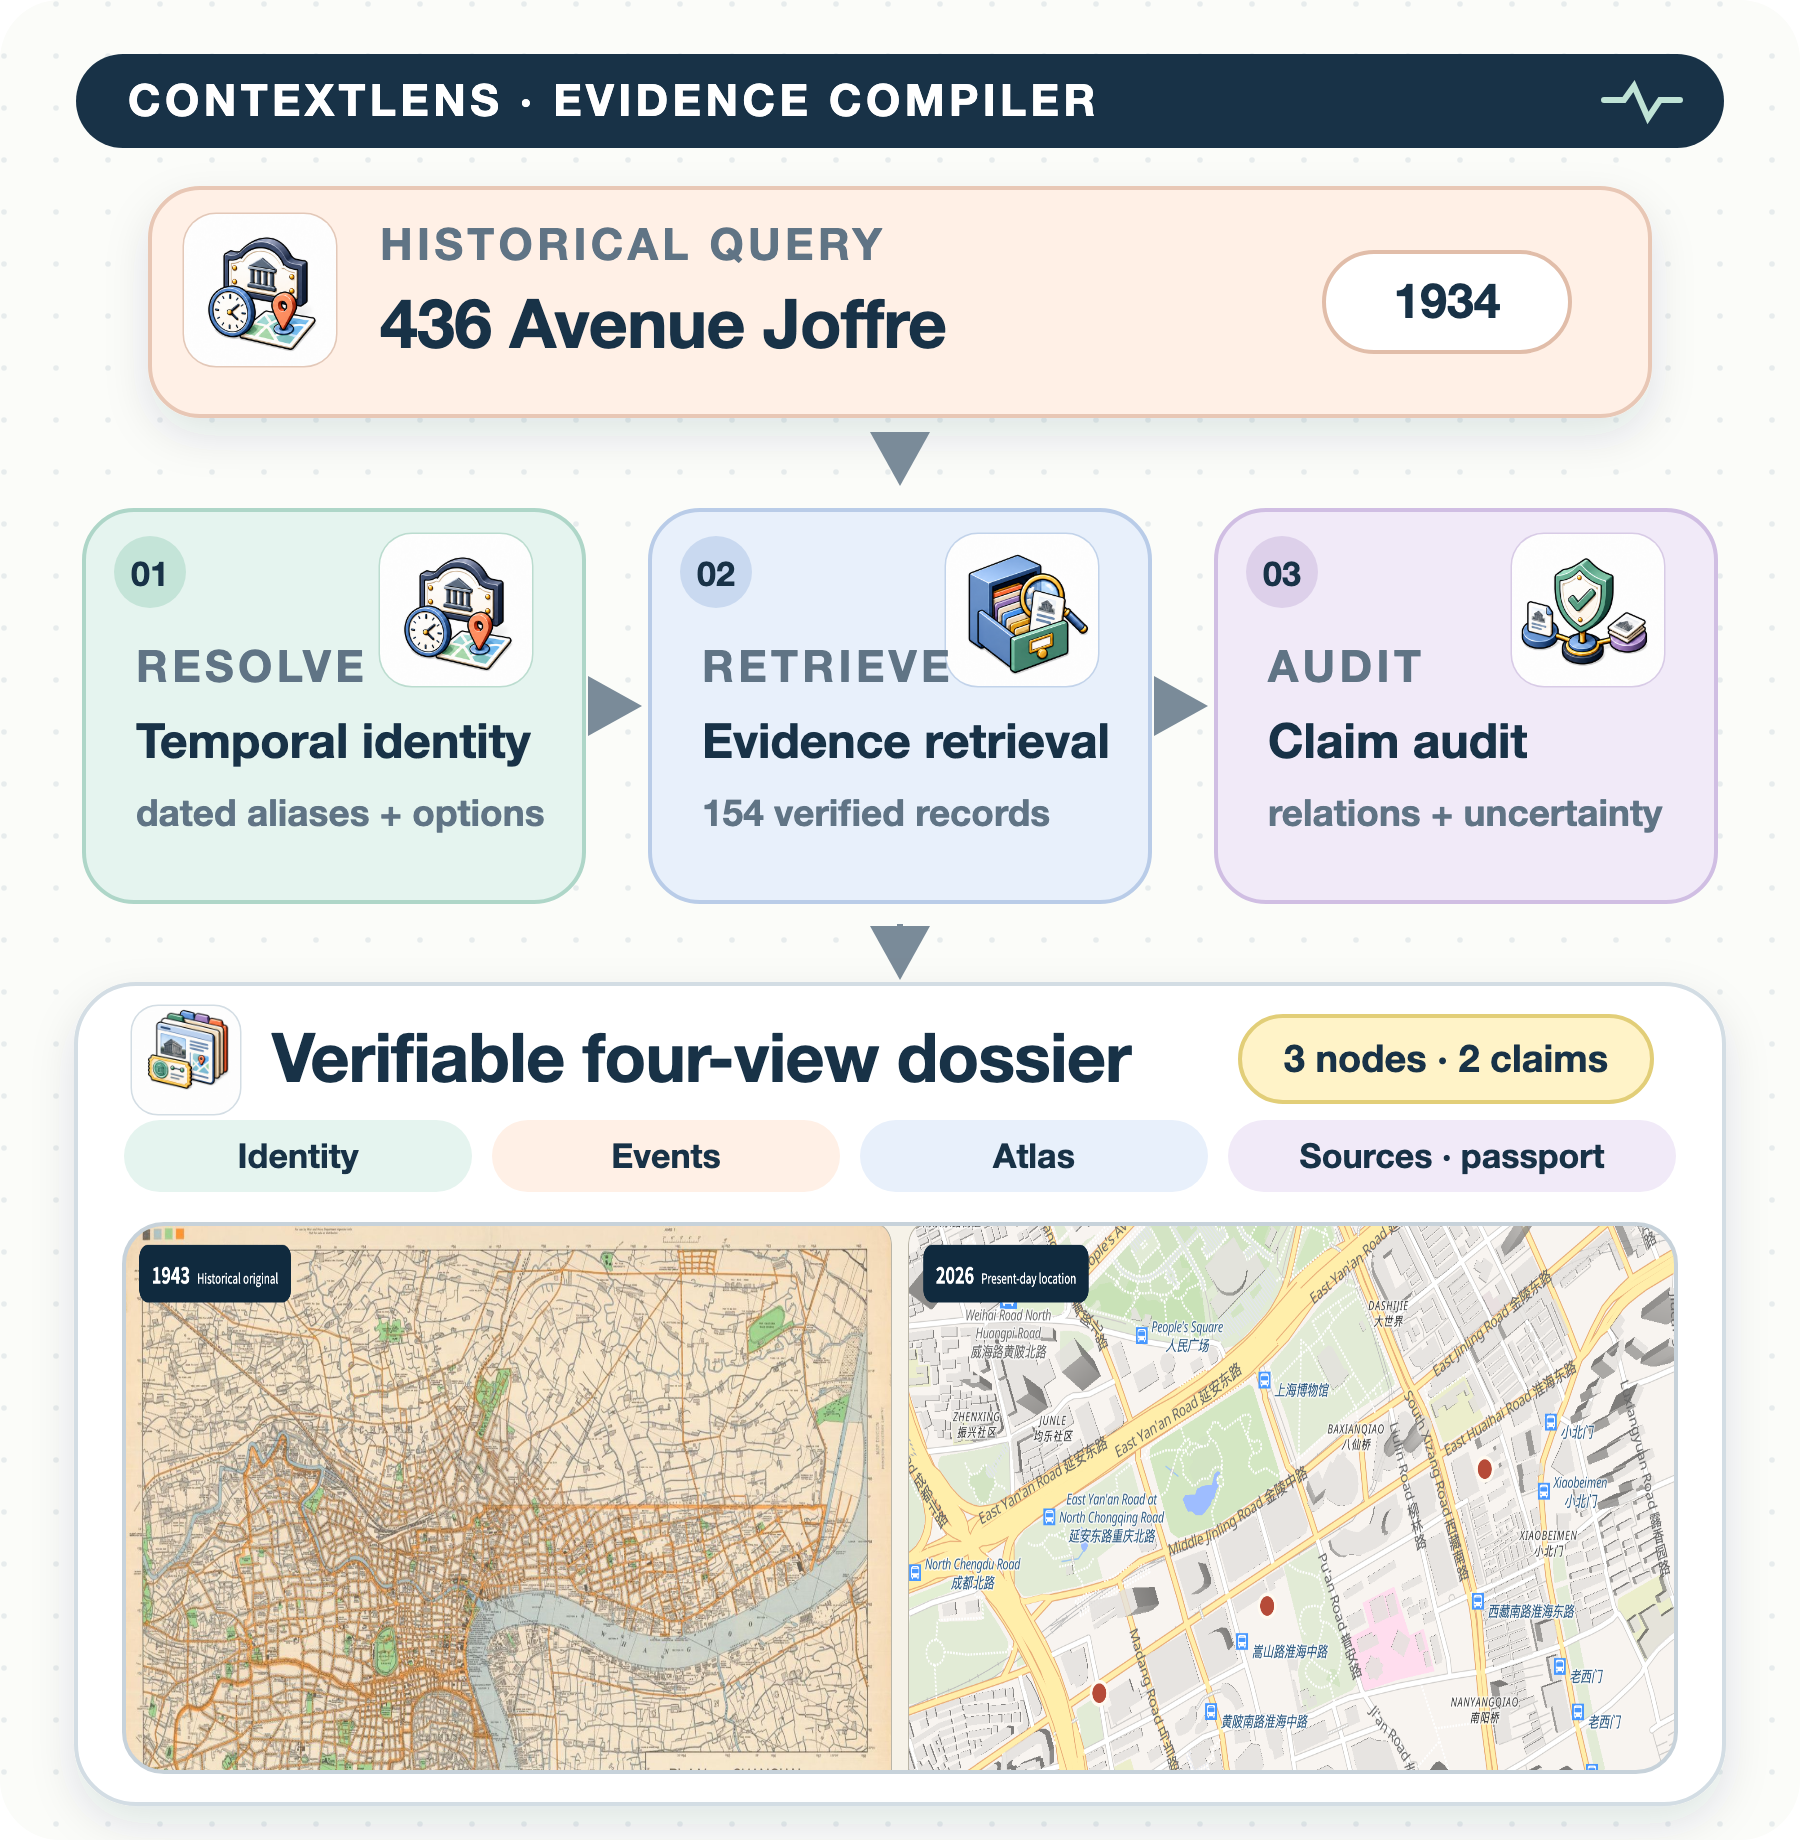
\includegraphics[height=0.76\textheight]{contextlens_teaser.png}
\end{columns}
\sourcefoot{System design and teaser: ContextLens AAAI-27 demonstration paper.}
\note{Explain the three contributions. Provenance validation and claim admission remain explicit system operations.}
\end{frame}

\section{System}

\begin{frame}[t]{\icontitle{Evidence compiler: four controlled stages}{compiler-stages.pdf}}
\centering
\vspace{0cm}
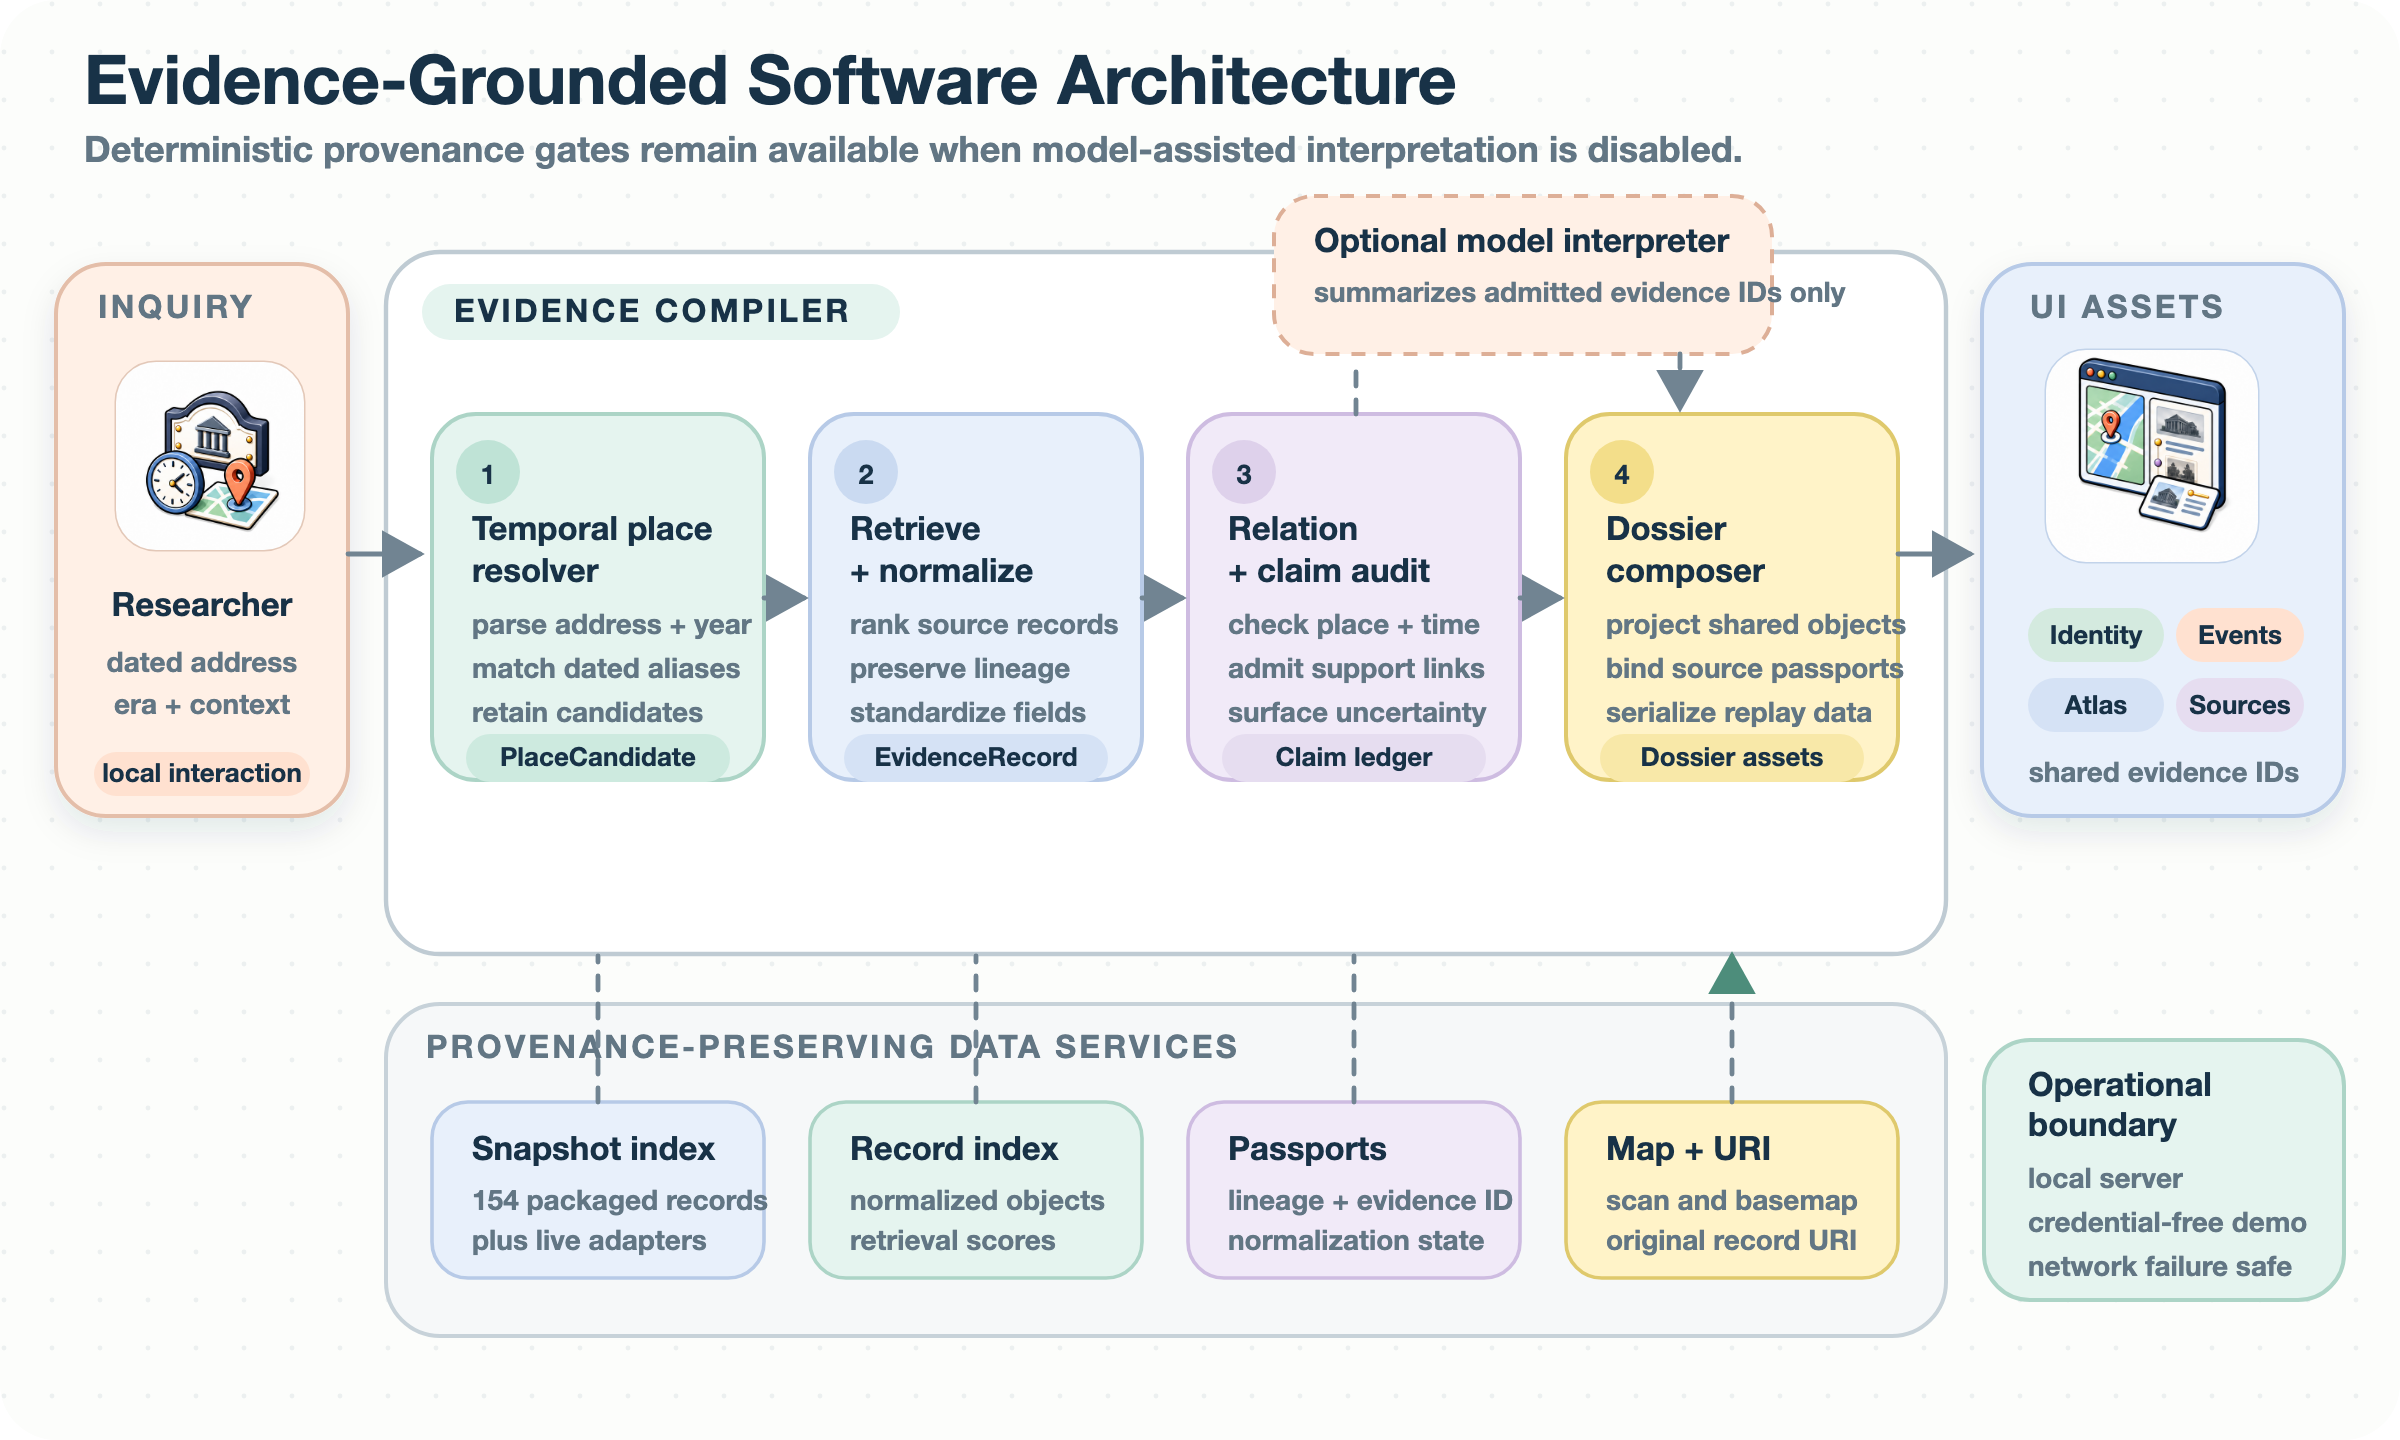
\includegraphics[width=\linewidth,trim={0 500 0 175},clip]{contextlens_architecture.png}
\makebox[0pt][l]{\raisebox{0pt}[0pt][0pt]{%
  \begin{tikzpicture}[remember picture,overlay]
    \node[anchor=center,fill=CalloutFill,draw=CalloutBorder,
      dashed,line width=0.65pt,rounded corners=4pt,
      minimum width=4.05cm,minimum height=1.02cm,
      inner xsep=0.18cm,inner ysep=0.09cm,align=center]
      at ([xshift=10.02cm,yshift=-1.85cm]current page.north west) {%
        \begin{minipage}{3.55cm}
          \centering
          {\fontsize{7.5}{8.4}\selectfont\bfseries\color{TeamInk}
            Optional model interpreter\par}
          \vspace{0.03cm}
          {\fontsize{6.4}{7.2}\selectfont\bfseries\color{PaperGray}
            Summarizes admitted\\evidence IDs only}
        \end{minipage}};
  \end{tikzpicture}}}%

\vspace{-0.36cm}
\claimbox{\small\textbf{Control boundary:} The optional model interpreter receives only evidence IDs admitted after relation and claim auditing.}
\sourcefoot{Technical Supplement, Figure A1.}
\note{Walk from the dated inquiry through resolution, normalization, claim audit, and dossier composition. Point to the optional model boundary.}
\end{frame}

\begin{frame}[t]{\icontitle{Provenance across seven pipeline stages}{provenance-chain.pdf}}
\centering
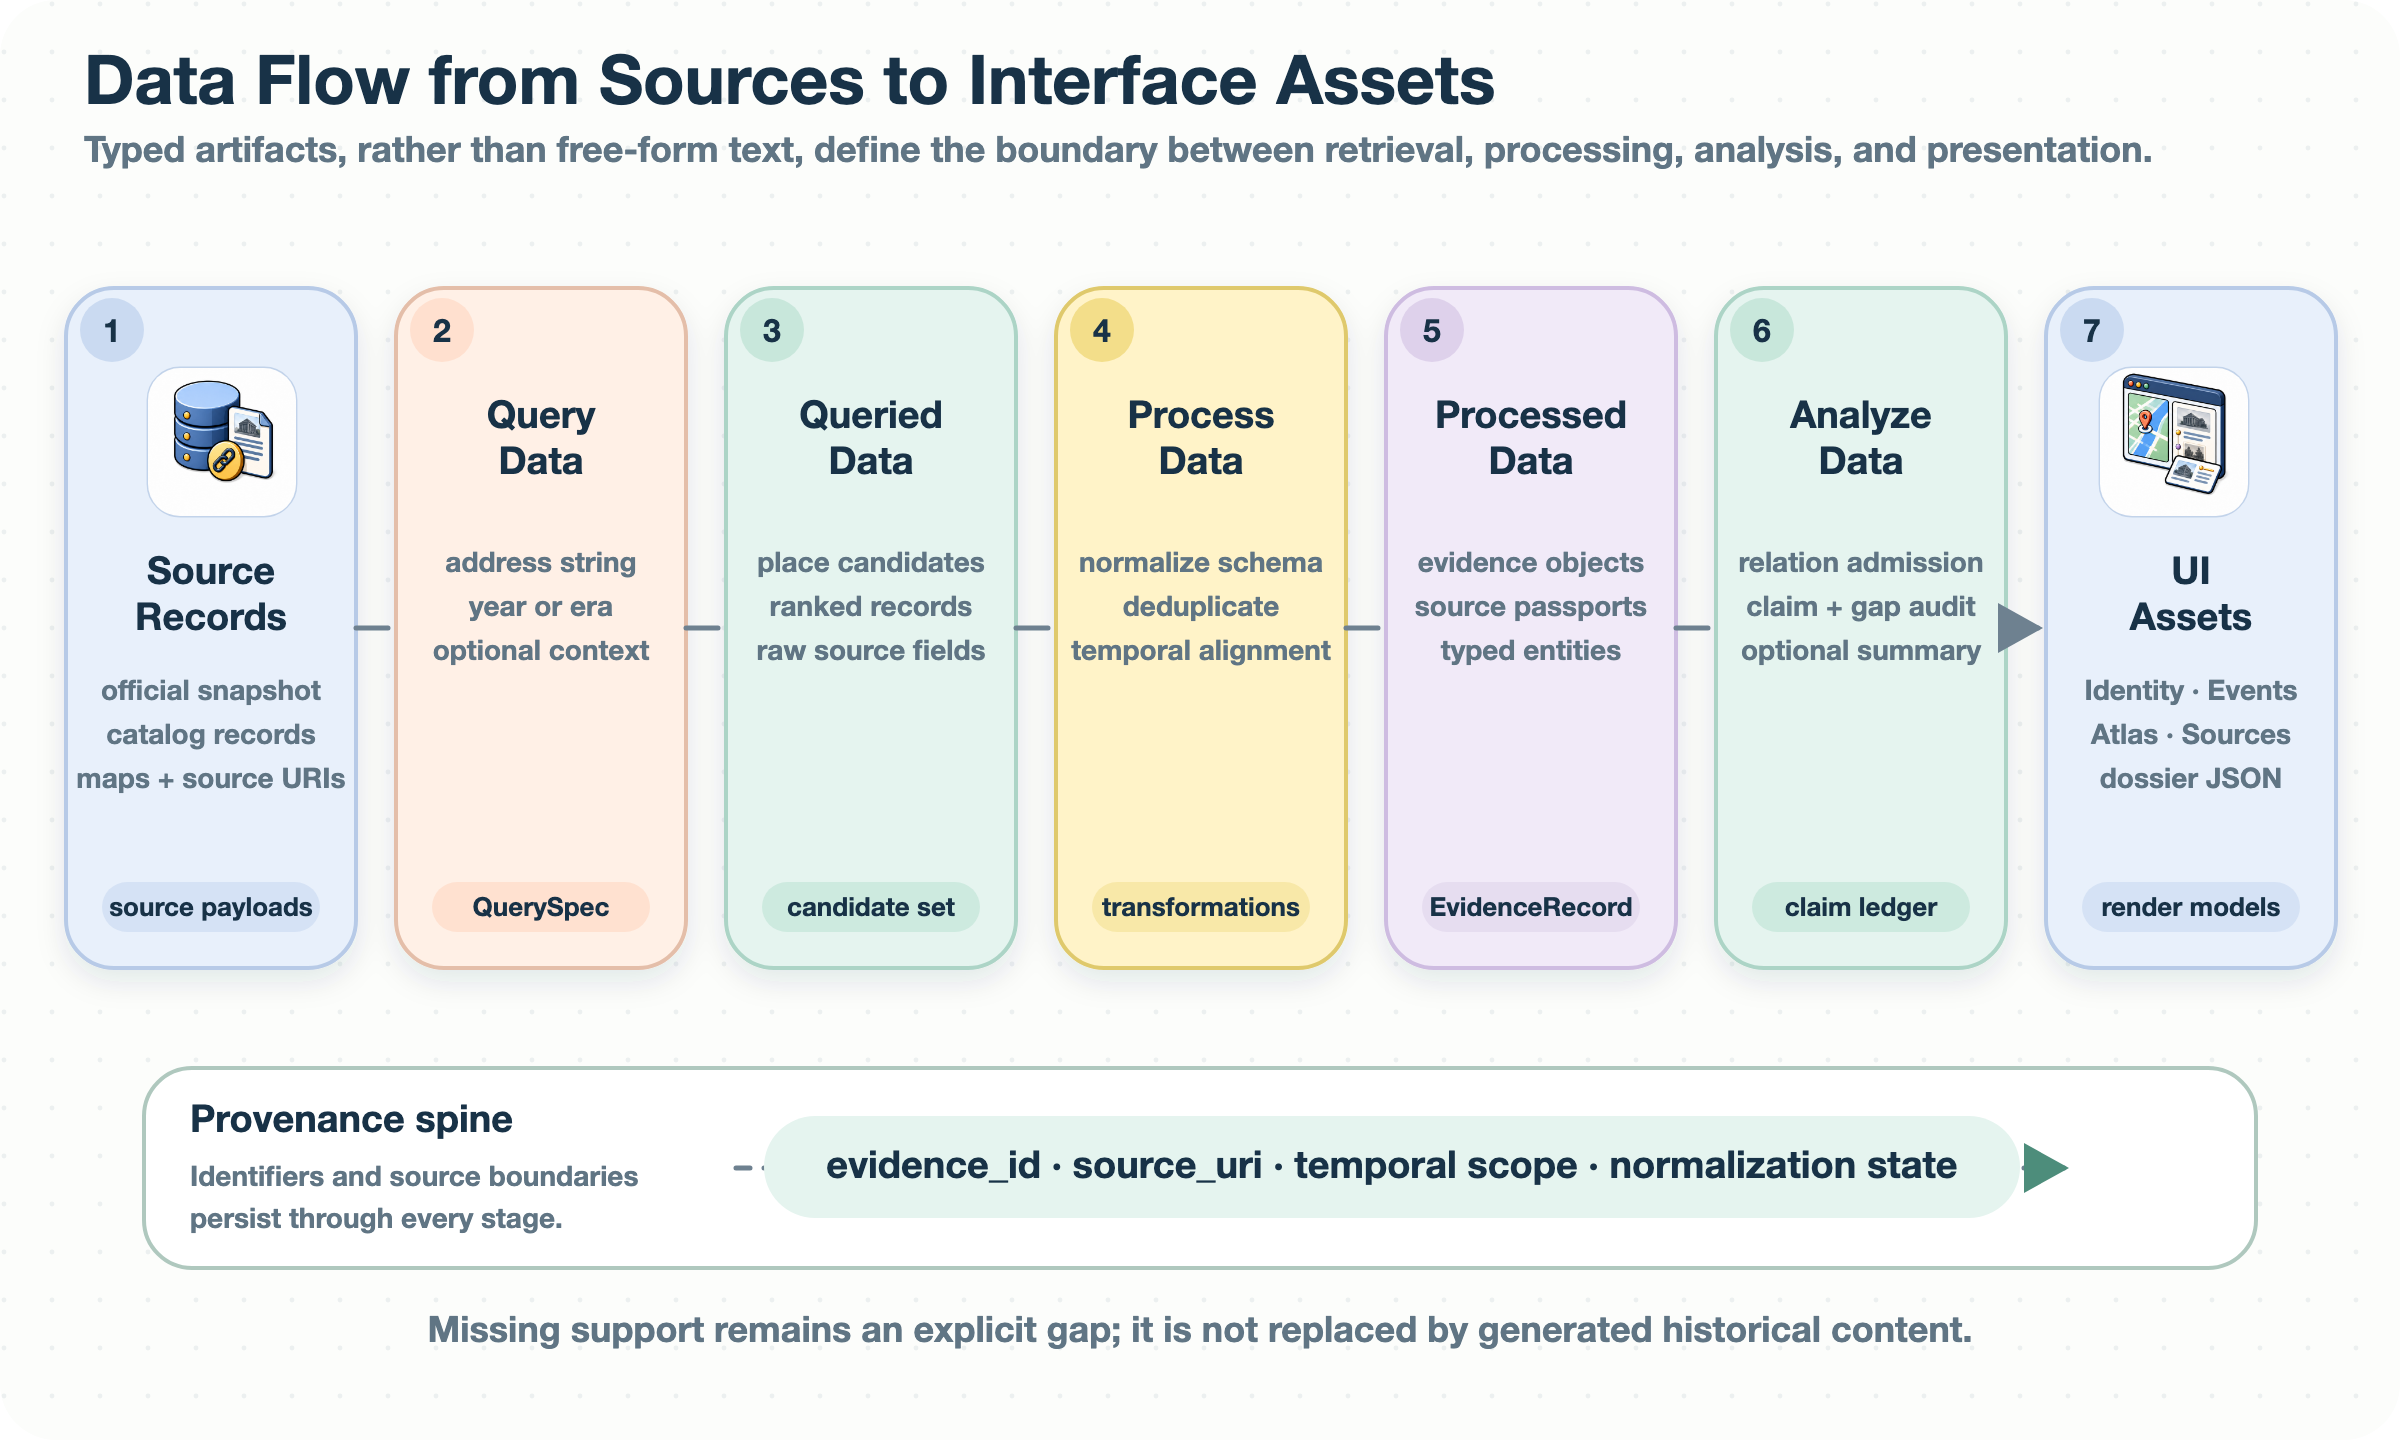
\includegraphics[width=\linewidth,trim={35 420 35 170},clip]{contextlens_data_flow.png}

\vspace{0em}
{\small\bfseries\color{DukeRoyalBlue}
Evidence ID, source URI, temporal scope, and normalization state persist across every stage.}
\sourcefoot{Technical Supplement, Figure A2. Current snapshot: 154 verified records.}
\note{The same evidence identifier survives retrieval, normalization, claim auditing, and interface rendering.}
\end{frame}

\section{Demonstration}

\begin{frame}[t]{\icontitle{Demo case: 436 Avenue Joffre in 1934}{address-dossier.pdf}}
\centering
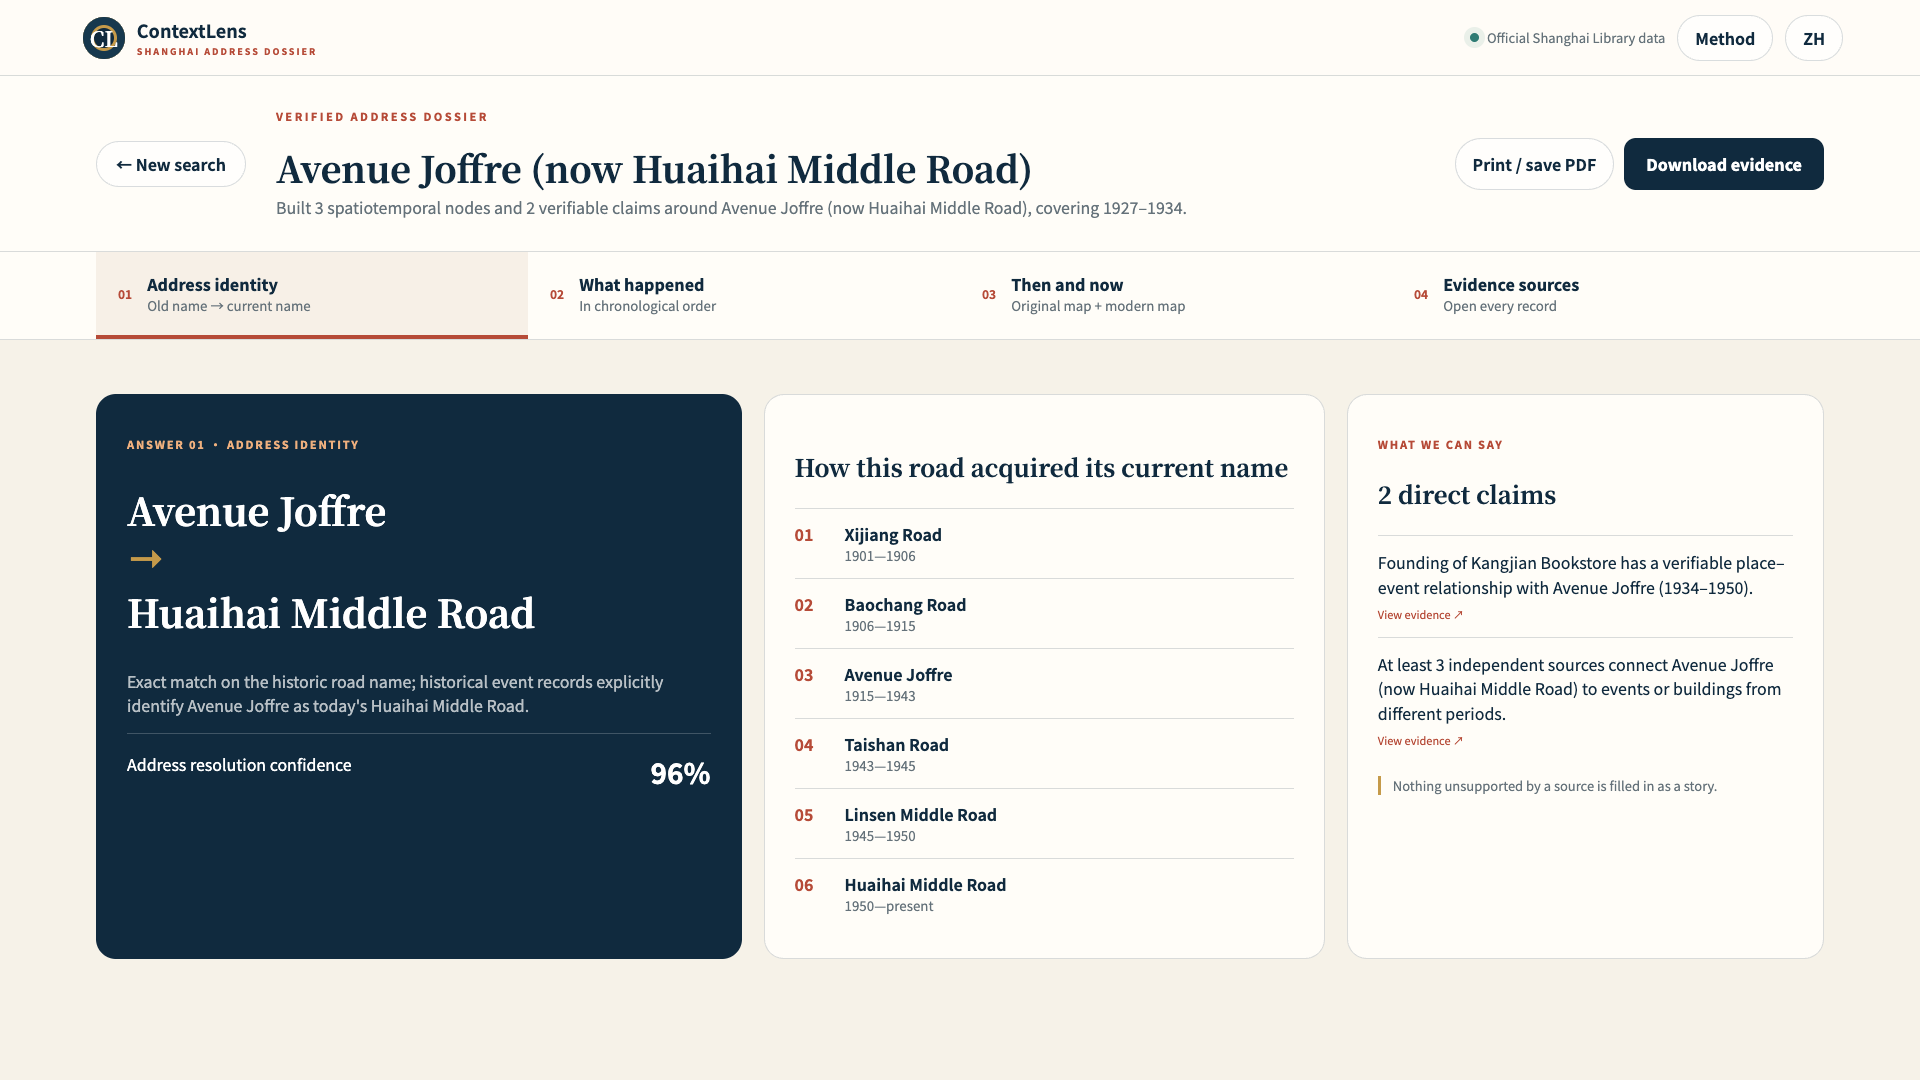
\includegraphics[width=0.98\linewidth,trim={0 90 0 120},clip]{ui_identity_en.png}
\sourcefoot{Current code capture, 10 September 2026: 96\% address-resolution confidence, six dated names, and two direct claims.}
\note{Clarify that 96 percent is resolver confidence for this case, not system-wide accuracy. Trace the road-name sequence from 1901 to the present.}
\end{frame}

\begin{frame}[t]{\icontitle{Evidence-bounded events and spatial context}{event-map.pdf}}
\begin{columns}[T,onlytextwidth]
\column{0.38\textwidth}
\centering
\textcolor{DukeRoyalBlue}{\textbf{Three evidence-linked nodes}}

\vspace{0.15em}
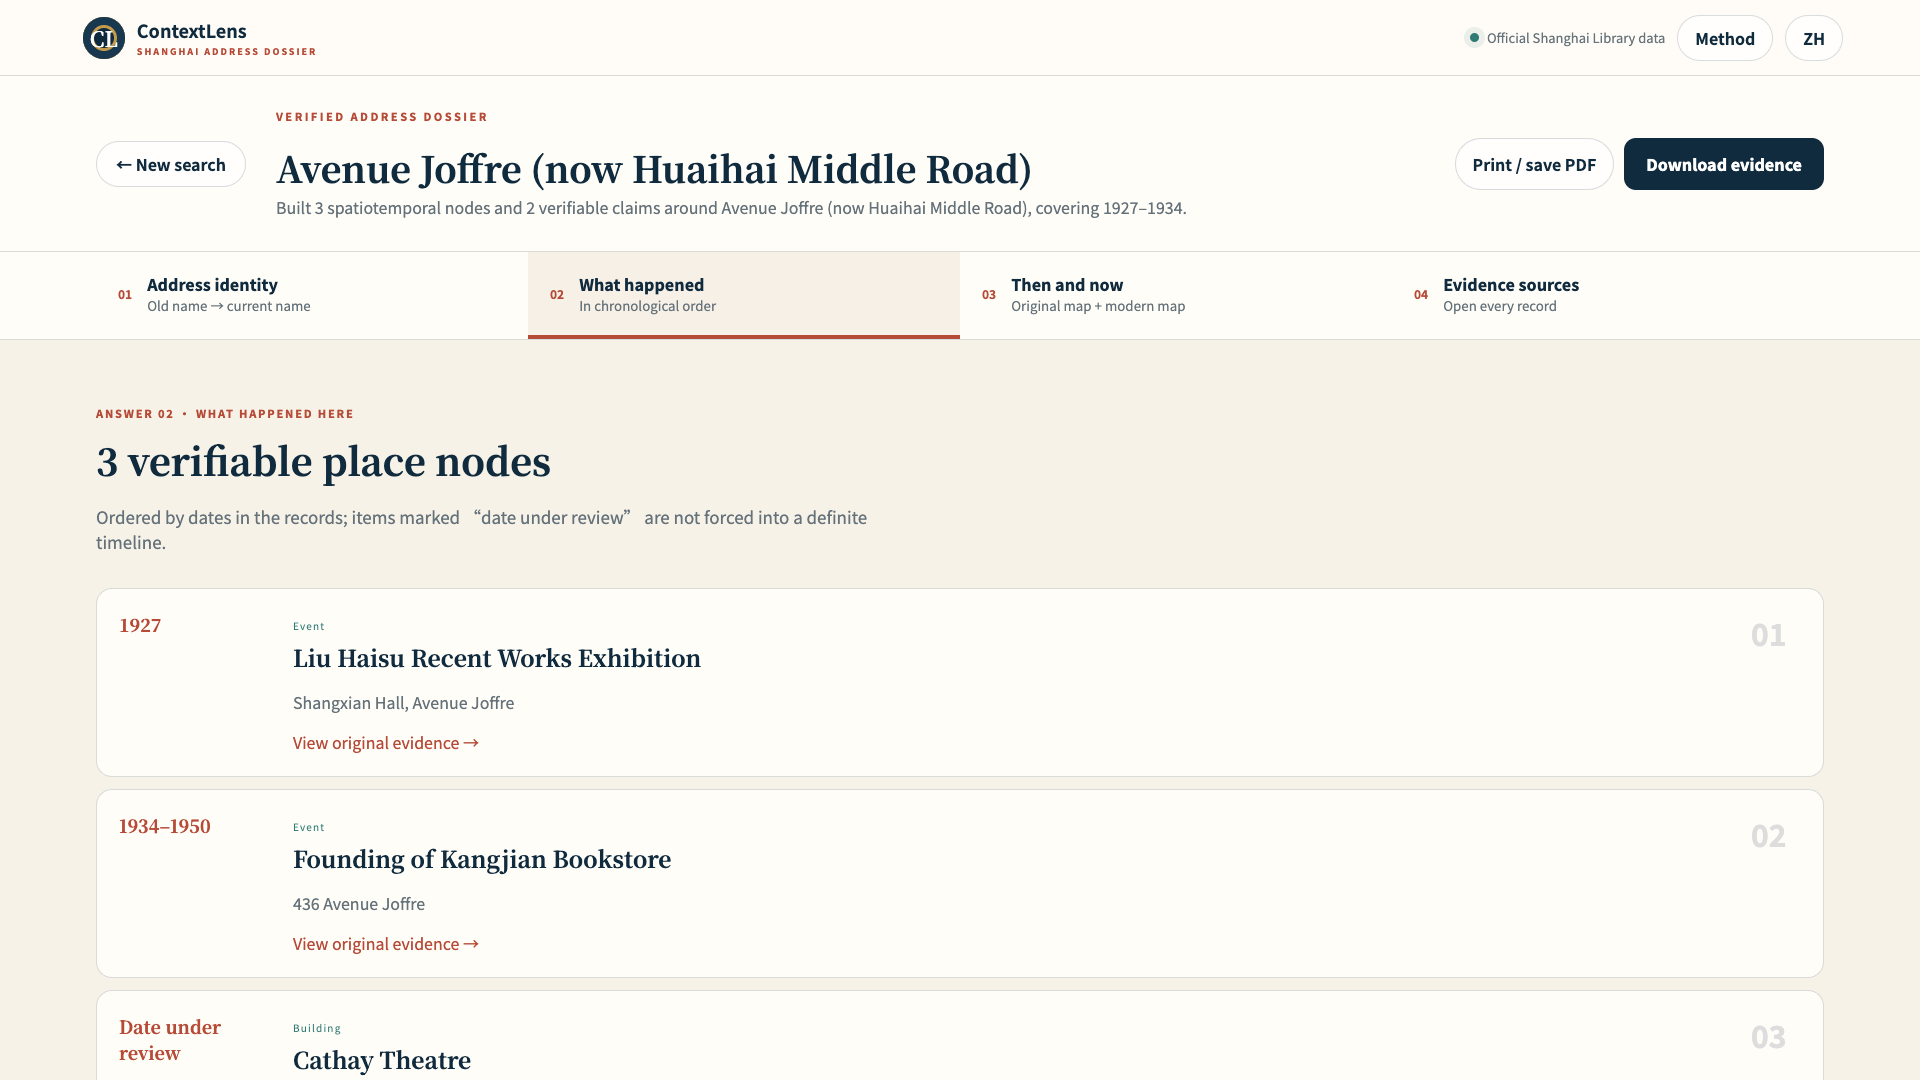
\includegraphics[width=0.90\linewidth,trim={0 0 650 0},clip]{ui_events_en.png}

\vspace{0.15em}
\small 1927: Liu Haisu exhibition\\
1934--1950: Kangjian Bookstore\\
Undated: Cathay Theatre under review

\column{0.58\textwidth}
\centering
\textcolor{DukeRoyalBlue}{\textbf{Two distinct map roles}}

\vspace{0.15em}
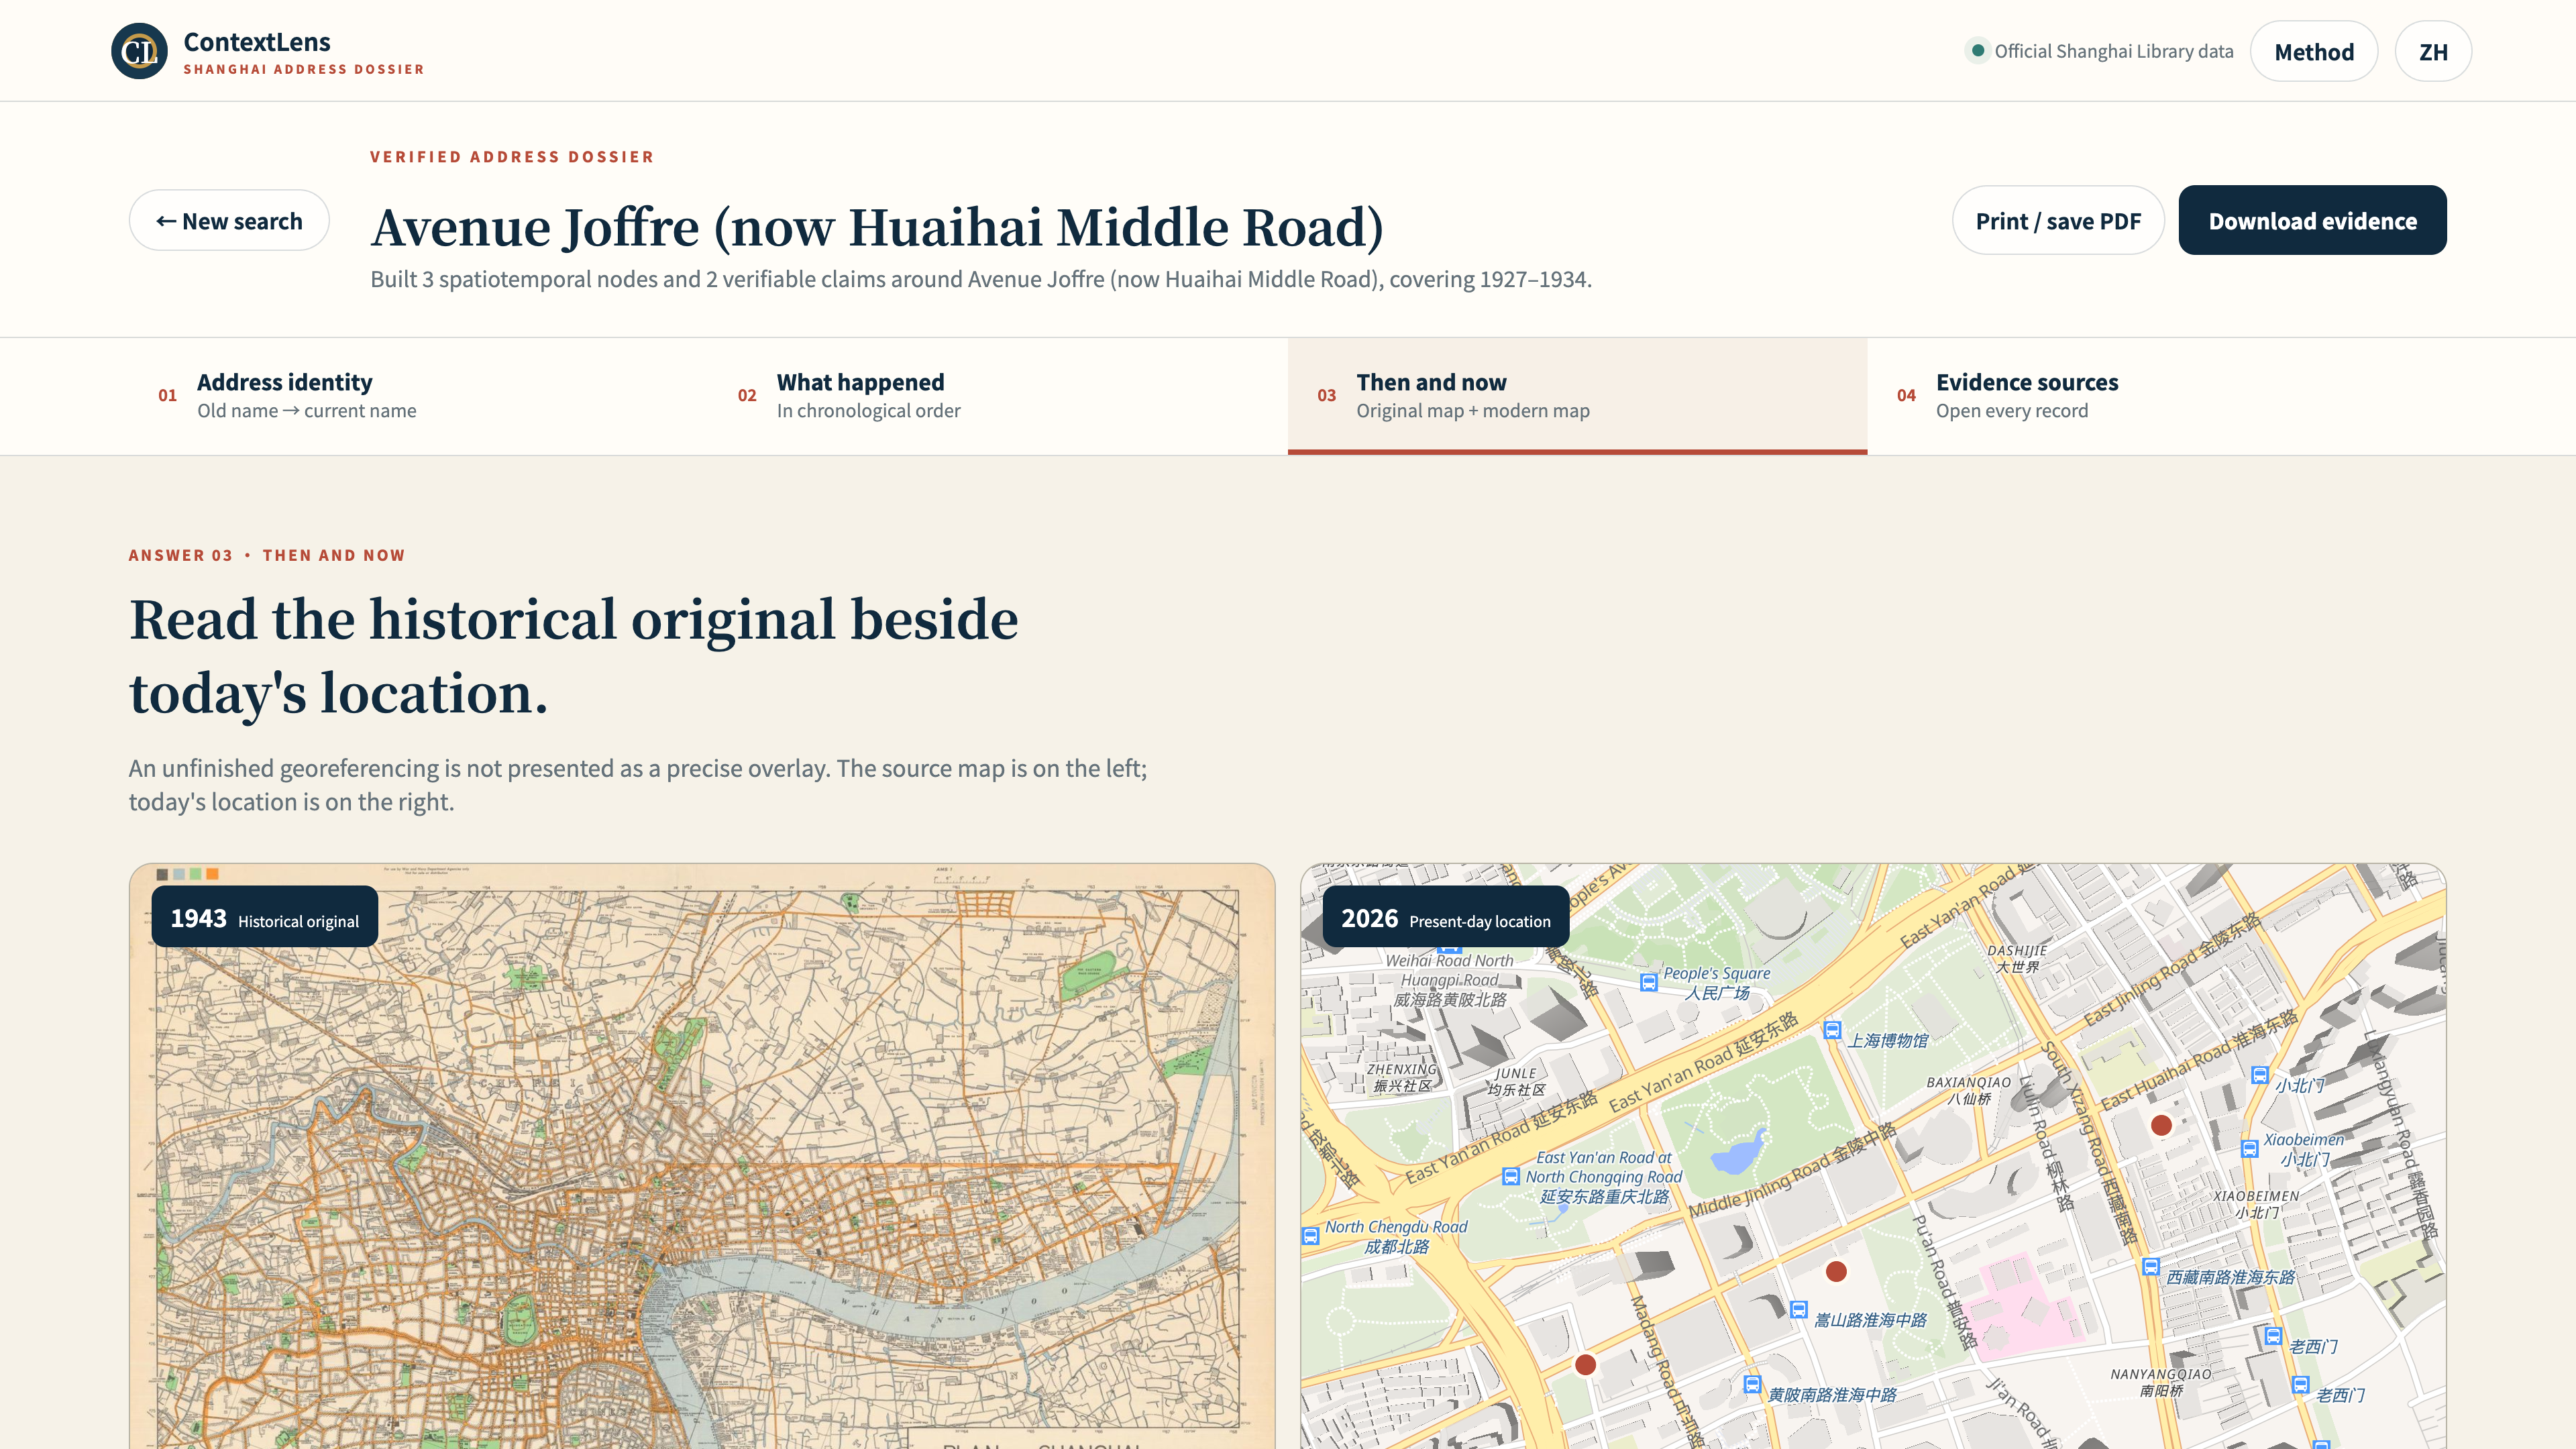
\includegraphics[width=0.94\linewidth]{contextlens_atlas.png}

\vspace{0.15em}
\small The 1943 scan supports visual orientation. The current map locates the resolved address. Exact house-number alignment remains unverified.
\end{columns}
\sourcefoot{Current Events view. Paper and interface Atlas view.}
\note{Separate dated events from records whose date remains under review. Explain why the archival scan and contemporary map have different evidentiary roles.}
\end{frame}

\begin{frame}[t]{\icontitle{Source Passports link claims to original records}{source-passport.pdf}}
\begin{columns}[T,onlytextwidth]
\column{0.52\textwidth}
\smalllead{A claim and its evidence card share one identifier}

\vspace{0.28em}
For the Kangjian Bookstore claim, the interface exposes:
\begin{itemize}
  \item Shanghai Library and the Historical and Cultural Events dataset.
  \item the 1934--1950 temporal scope.
  \item evidence ID \texttt{event-kangjian-1934}.
  \item normalization state and original URI.
\end{itemize}

\vspace{0.25em}
{\small\bfseries\color{DukeRoyalBlue}The normalized record preserves the source boundary.}

\column{0.44\textwidth}
\centering
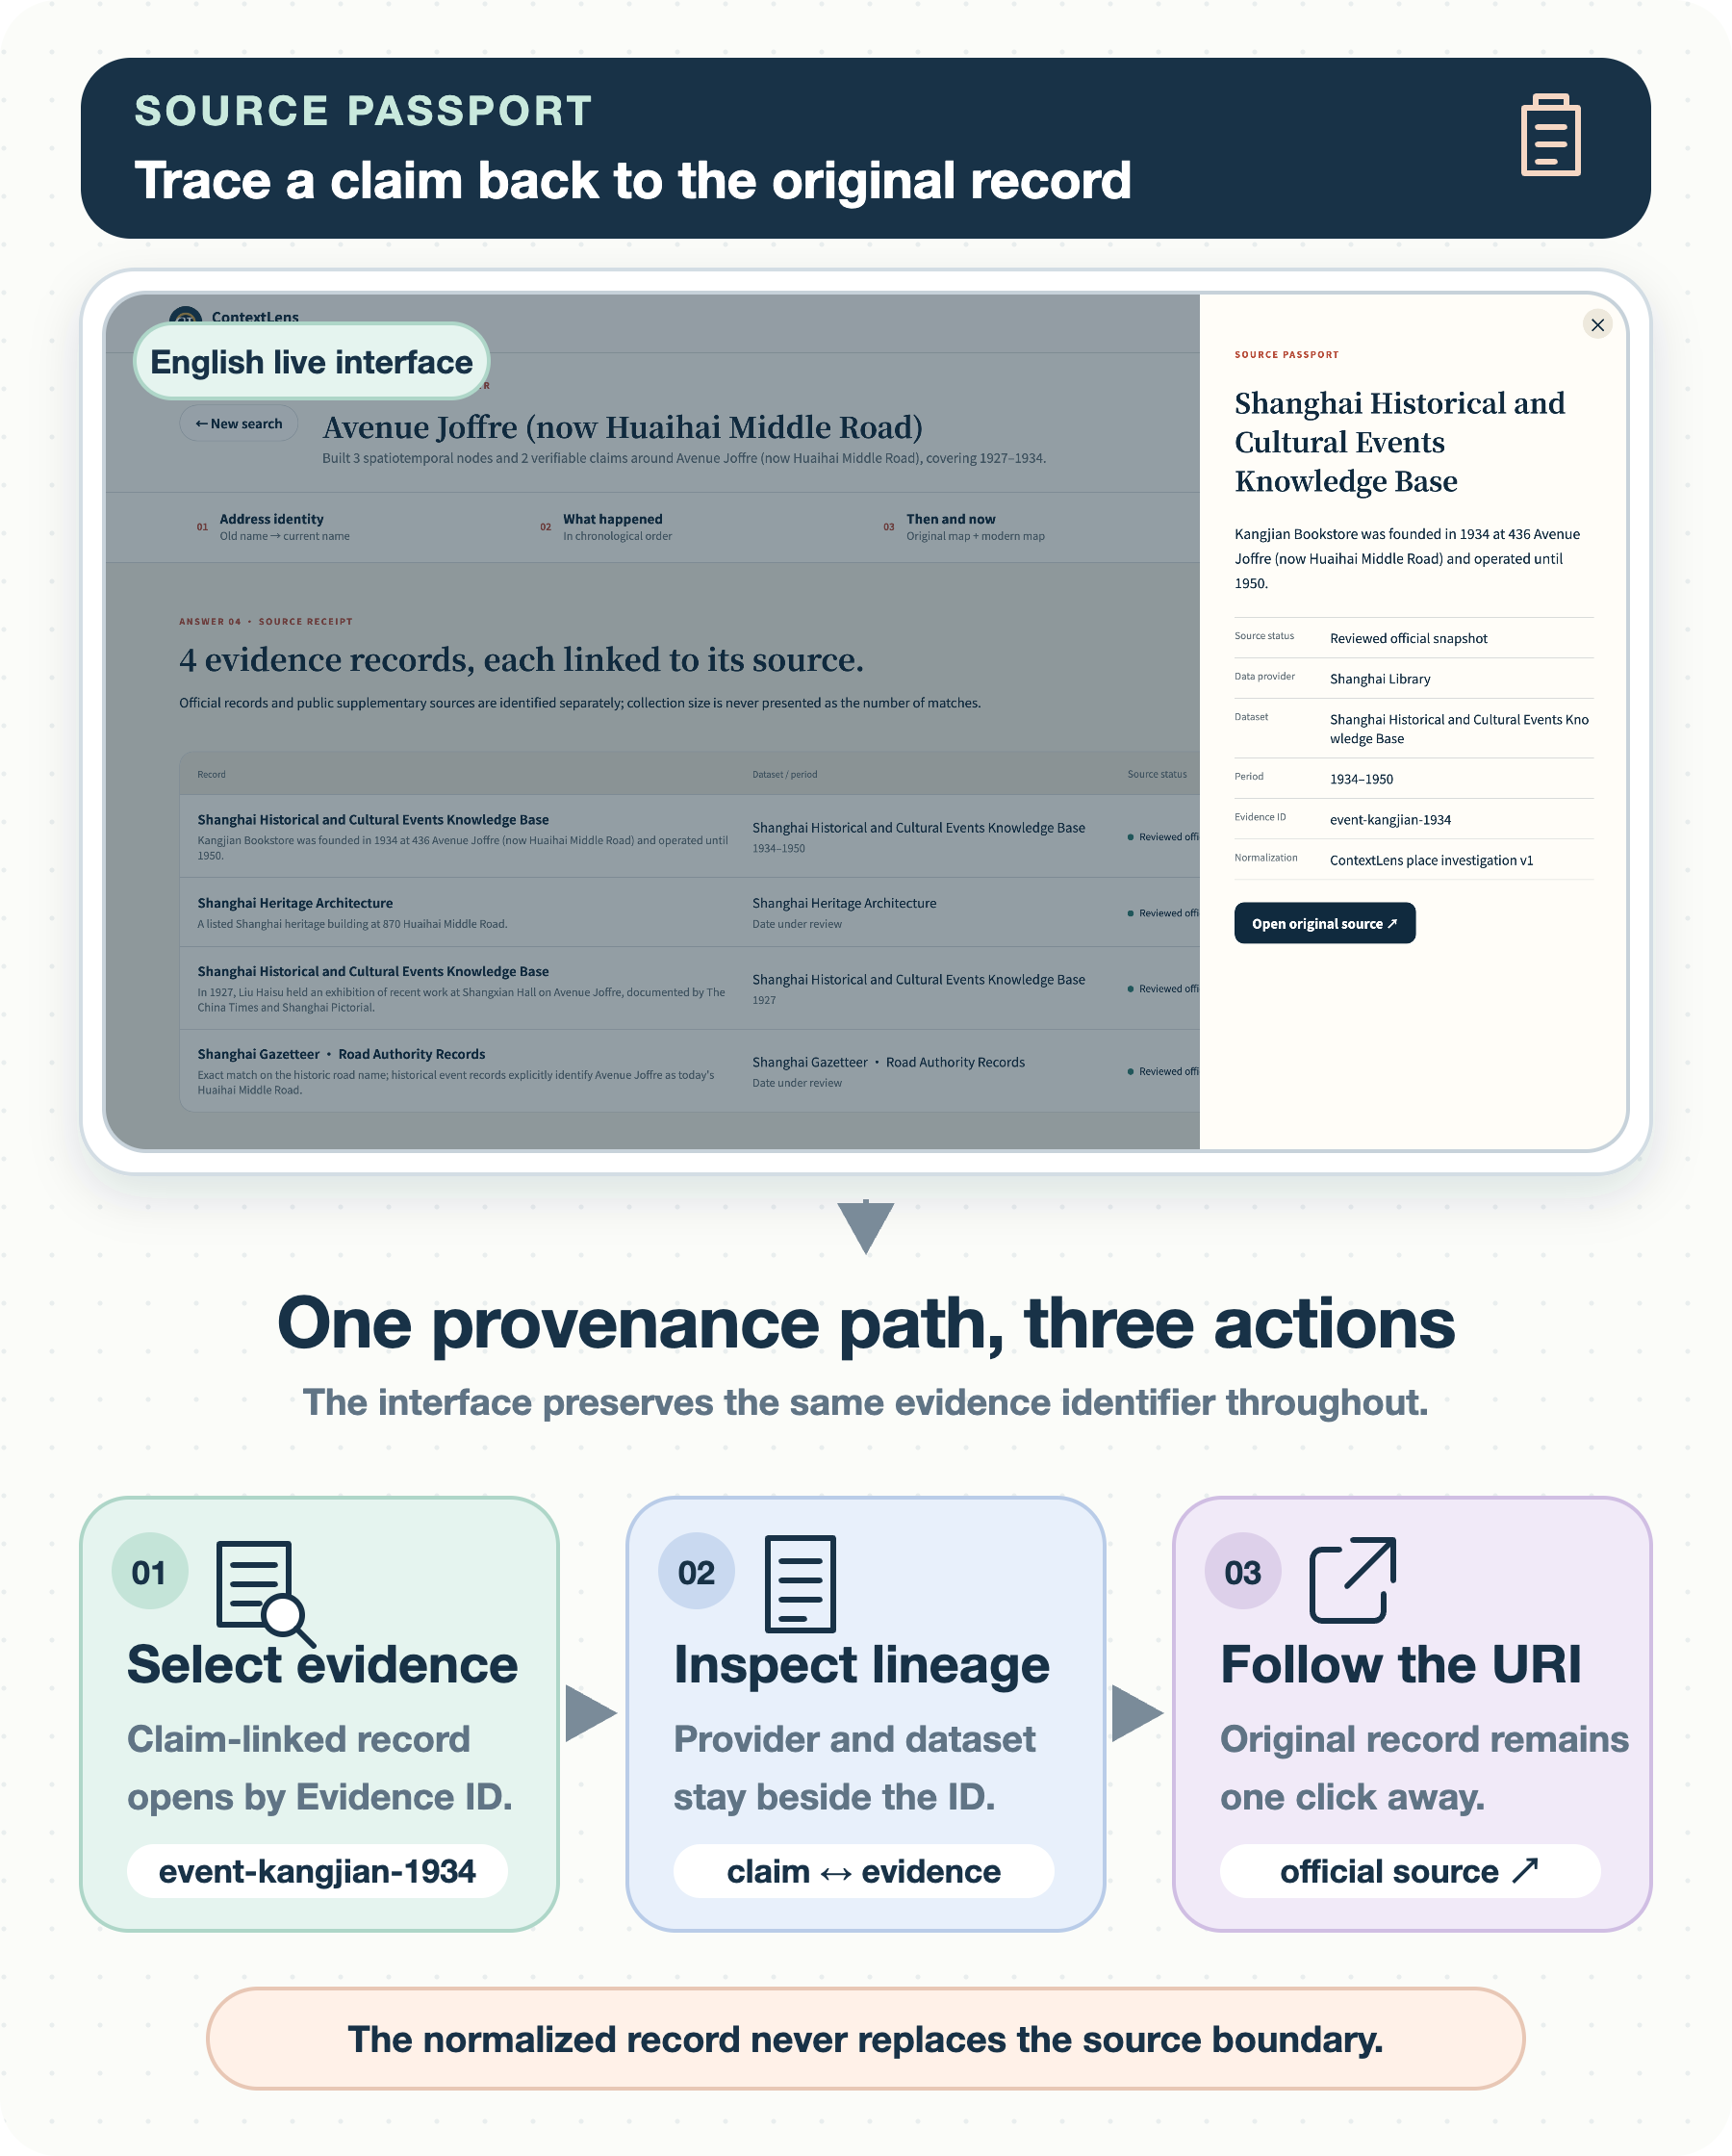
\includegraphics[height=0.70\textheight]{contextlens_sources_figure.png}
\end{columns}
\sourcefoot{AAAI paper, Figure 2. Current Source Passport fields.}
\note{Open the Source Passport slowly. Point out the provider, dataset, period, evidence ID, normalization, and original source link.}
\end{frame}

\begin{frame}[t]{\icontitle{Explicit ambiguity and unresolved states}{ambiguity-branches.pdf}}
\small
\centering
\smalllead{The system treats uncertainty as an output state}

\vspace{0.35em}
\renewcommand{\arraystretch}{1.28}
\begin{tabularx}{\textwidth}{>{\bfseries}p{0.14\textwidth}p{0.22\textwidth}X p{0.22\textwidth}}
\rowcolor{DukeRoyalBlue}
\color{white}Input state & \color{white}\textbf{Example} & \color{white}\textbf{System response} & \color{white}\textbf{Claim behavior}\\
\rowcolor{SoftBlue}
Resolved & 436 Avenue Joffre, 1934 & One temporally compatible candidate & Admit two direct claims\\
Ambiguous & Nanjing Road department store & Retain East and West Nanjing Road candidates & Request more context\\
\rowcolor{SoftBlue}
Unresolved & 9999 Mars Road & Return unresolved and ask for evidence & Generate no historical fact\\
\end{tabularx}

\vspace{0.25em}
\claimbox{\centering\textbf{No candidate, no claim. Competing candidates remain available for review.}}
\sourcefoot{AAAI paper, Demonstration Scenario. Current tests for ambiguity and negative cases.}
\note{Use the Nanjing Road ambiguity and the synthetic Mars Road negative control to show that the system does not force a confident answer.}
\end{frame}

\section{Evaluation}

\begin{frame}[t]{\icontitle{Implementation and verification}{audit-ledger.pdf}}
\footnotesize
\begin{columns}[T,onlytextwidth]
\column{0.30\textwidth}
\metric{154}{verified snapshot records}
\vspace{0.22em}
\metric{0}{demo-seed records on the reviewed path}
\vspace{0.22em}
\metric{29}{local Python test functions passed}

\column{0.65\textwidth}
\textcolor{DukeRoyalBlue}{\textbf{Implementation}}
\begin{itemize}
  \setlength{\itemsep}{1pt}
  \item Python controller with a deterministic evidence compiler
  \item TypeScript UI, local HTTP API, and SQLite evidence index
  \item Credential-free local run with optional live adapters
  \item Model assistance occurs after relation and claim auditing
\end{itemize}

\vspace{0.18em}
\textcolor{DukeRoyalBlue}{\textbf{Verified behavior}}
\begin{itemize}
  \setlength{\itemsep}{1pt}
  \item dated address resolution, ambiguity, and negative cases
  \item relation gating and evidence-bounded model citations
  \item network failure, TLS, and privacy-safe audit logs
  \item asynchronous states and interface contracts
\end{itemize}
\end{columns}
\vspace{0em}
\claimbox{\small\textbf{Interpretation:} These checks verify implementation behavior. They do not establish retrieval accuracy or user-study outcomes.}
\sourcefoot{Current README, application architecture, local health response, and tests re-run on 10 September 2026.}
\note{Present the test count as an implementation check. Do not call it accuracy, effectiveness, or user validation.}
\end{frame}

\begin{frame}[t]{\icontitle{Scope and evaluation agenda}{scope-boundary.pdf}}
\begin{columns}[T,onlytextwidth]
\column{0.47\textwidth}
\textcolor{GoodGreen}{\large\textbf{Supported in the current demo}}
\begin{itemize}
  \item Shanghai-specific packaged snapshot
  \item inspectable evidence and Source Passports
  \item explicit ambiguity and unresolved states
  \item offline interaction and failure-safe dossier output
\end{itemize}

\column{0.49\textwidth}
\textcolor{WarnOrange}{\large\textbf{Open research questions}}
\begin{itemize}
  \item resolution quality across a broader address benchmark
  \item expert correction workflows and historian evaluation
  \item claim-citation precision and contradiction handling
  \item more precise georeferencing for historical maps
\end{itemize}
\end{columns}

\vspace{0.28em}
\claimbox{\centering\textbf{ContextLens is an investigation interface, not a general historical geocoder.}}

\vspace{0em}
\centering\small Some coordinates remain coarse. The system has not yet completed a historian or public-user study.
\sourcefoot{AAAI paper, Design Boundaries and Scope.}
\note{State the limits directly. The next evaluation should measure resolver quality, claim-citation precision, expert correction, and user usefulness.}
\end{frame}


\begin{frame}[c]{\icontitle{Acknowledgments}{support-network.pdf}}
\begin{columns}[c,onlytextwidth]
\column{0.24\textwidth}
\centering

\includegraphics[width=2.45cm]{project-bridge.pdf}

\vspace{0.18cm}
{\scriptsize\color{PaperGray}\bfseries Related foundations,\par distinct deliverables}

\column{0.71\textwidth}
{\large\bfseries\color{DukeNavyBlue}Project and scholarship support}\par
\vspace{0.24cm}
\begin{beamercolorbox}[wd=\linewidth,sep=10pt,rounded=true]{block body}
  {\small Sean Wan, Shilin Ou, Yutian Wang, and Polina Postnikova acknowledge
  support from the Summer Research Scholars Program at Duke Kunshan University
  and the DKU Library grant for the Shanghai Library Open Data Contest project
  \textbf{StableTradeAtlas}, supervised by Prof. Luyao Zhang.}
\end{beamercolorbox}

\vspace{0.18cm}
\begin{beamercolorbox}[wd=\linewidth,sep=8pt,rounded=true,center]{project distinction}
  {\small\bfseries ContextLens was developed beyond the contest as a separate
  intelligent research and demonstration deliverable.}
\end{beamercolorbox}
\end{columns}
\end{frame}


\begin{frame}[plain]
\stacanvas
\vspace*{0.72cm}
\centering
{\fontsize{32}{36}\selectfont\bfseries\color{AtlasBlue}StableTradeAtlas
  \staoverviewclip{trade-atlas.pdf}}\par
\vspace{0.16cm}
{\fontsize{15}{18}\selectfont\color{AtlasBlue}
Shanghai Library Open Data Contest 2026}\par
\vspace{0.20cm}

\begin{tikzpicture}
  \shade[left color=TeamPurple,right color=TeamGreen] (0,0) rectangle (7.1cm,0.07cm);
\end{tikzpicture}\par
\vspace{0.20cm}
{\fontsize{14}{16.5}\selectfont\bfseries\color{TeamGreen}DKU Team:}\par
\vspace{0.08cm}
{\fontsize{12.5}{15}\selectfont\color{TeamGreen}
\textbf{Lead and Co-lead:} Sean Wan and Shilin Ou\par
\textbf{Members:} Claire Wang, Polina Postnikova\par
\textbf{Faculty Mentor:} Prof. Luyao Zhang\par}
\vspace{0.16cm}
{\fontsize{13.5}{16}\selectfont\bfseries\color{TeamInk}Acknowledgments:}\par
\vspace{0.05cm}
{\fontsize{11.5}{14}\selectfont\color{TeamInk}
\textbf{External Advisers:} Shiping Chen, Dongping Liu, Xuechao Wang}
\end{frame}

\section{Team}

\begin{frame}[plain,t]
\stacanvas
\staheading{StableTradeAtlas Team Profile: Sean Wan}{Project Lead / Agent Architecture / Trustworthy Evaluation}{agent-architecture.pdf}
\vspace*{1.36cm}
\begin{columns}[T,onlytextwidth]
  \column{0.21\textwidth}
  \centering
  \profilephoto{team_original/sean_wan.jpg}{1.24cm}{2.75cm}{-0.10cm}

  \vspace{0.13cm}
  {\fontsize{14}{16}\selectfont\bfseries\color{AtlasBlue}Sean Wan}\par
  \vspace{0.06cm}
  {\fontsize{8.8}{10.5}\selectfont\color{PaperGray}
  Project leadership and trustworthy agent evaluation}

  \column{0.75\textwidth}
  \profilelabel{Contribution highlight}
  {\fontsize{9.2}{11.1}\selectfont
  Sean leads StableTradeAtlas's trustworthy-agent architecture. His StableEval
  Arena experience informs prediction-quality, risk, and evidence-aware evaluation.}

  \vspace{0.16cm}
  \begin{columns}[T,onlytextwidth]
    \column{0.37\textwidth}
    \profilelabel{Relevant expertise}
    {\fontsize{8.3}{9.8}\selectfont
    \begin{itemize}
      \setlength{\itemsep}{1pt}
      \item Agentic AI evaluation and benchmarks
      \item RAG workflows and structured answers
      \item Cost, latency, citation, and risk auditing
      \item Full-stack MVP and GitHub coordination
    \end{itemize}}

    \column{0.60\textwidth}
    \profilelabel{Key contributions}
    {\fontsize{8.3}{9.8}\selectfont
    \begin{itemize}
      \setlength{\itemsep}{1pt}
      \item \textbf{Historical Evidence Compiler:} Connects old Shanghai addresses with traceable people, places, events, and documents.
      \item \textbf{Trustworthy AI:} Adds claim-level citations, uncertainty auditing, privacy protection, and evidence-based guardrails.
      \item \textbf{Spatiotemporal public experience:} Integrates historical maps, modern 3D geography, and bilingual interactive storytelling.
    \end{itemize}}
  \end{columns}
\end{columns}
\end{frame}

\begin{frame}[plain,t]
\stacanvas
\staheading{StableTradeAtlas Team Profile: Shilin Ou}{Blockchain Infrastructure / Security / Agent Audit Layer}{secure-audit.pdf}
\vspace*{1.36cm}
\begin{columns}[T,onlytextwidth]
  \column{0.21\textwidth}
  \centering
  \profilephoto{team_original/shilin_ou.jpg}{1.24cm}{2.75cm}{-0.10cm}

  \vspace{0.13cm}
  {\fontsize{14}{16}\selectfont\bfseries\color{AtlasBlue}Shilin Ou}\par
  \vspace{0.06cm}
  {\fontsize{8.8}{10.5}\selectfont\color{PaperGray}
  Secure infrastructure and auditable agent systems}

  \column{0.75\textwidth}
  \profilelabel{Contribution highlight}
  {\fontsize{9.2}{11.1}\selectfont
  Shilin brings SolarChain experience to a secure, modular, auditable evidence
  agent designed to extend beyond one prototype.}

  \vspace{0.16cm}
  \begin{columns}[T,onlytextwidth]
    \column{0.39\textwidth}
    \profilelabel{Relevant expertise}
    {\fontsize{8.5}{10.2}\selectfont
    \begin{itemize}
      \setlength{\itemsep}{1.5pt}
      \item SolarChain and blockchain infrastructure
      \item Secure data flows and audit design
      \item Agent reliability and technical-risk analysis
      \item System integration and prototype testing
    \end{itemize}}

    \column{0.58\textwidth}
    \profilelabel{Expected contribution}
    {\fontsize{8.5}{10.2}\selectfont
    \begin{itemize}
      \setlength{\itemsep}{1.5pt}
      \item Co-develop the agent architecture with Sean.
      \item Design audit checkpoints for API keys, logs, citations, and outputs.
      \item Develop the secure-agent and technical-risk narrative.
      \item Test the MVP workflow and document failure modes.
    \end{itemize}}
  \end{columns}
\end{columns}
\end{frame}

\begin{frame}[plain,t]
\stacanvas
\staheading{StableTradeAtlas Team Profile: Yutian (Claire) Wang}{Governance / Open-Source Community / Developer Ecosystem}{open-governance.pdf}
\vspace*{1.36cm}
\begin{columns}[T,onlytextwidth]
  \column{0.21\textwidth}
  \centering
  \profilephoto{team_original/yutian_wang.jpg}{1.24cm}{2.75cm}{-0.08cm}

  \vspace{0.13cm}
  {\fontsize{12.8}{14.8}\selectfont\bfseries\color{AtlasBlue}Yutian (Claire) Wang}\par
  \vspace{0.06cm}
  {\fontsize{8.8}{10.5}\selectfont\color{PaperGray}
  Governance and developer-community strategy}

  \column{0.75\textwidth}
  \profilelabel{Contribution highlight}
  {\fontsize{9.2}{11.1}\selectfont
  Claire brings a governance and developer-community perspective, moving the
  internal prototype toward a reproducible, open-source, public-facing AI application.}

  \vspace{0.16cm}
  \begin{columns}[T,onlytextwidth]
    \column{0.39\textwidth}
    \profilelabel{Related expertise}
    {\fontsize{8.5}{10.2}\selectfont
    \begin{itemize}
      \setlength{\itemsep}{1.5pt}
      \item DAO and decentralized governance research direction
      \item Open-source collaboration workflows
      \item Developer-community positioning and documentation
    \end{itemize}}

    \column{0.58\textwidth}
    \profilelabel{Key contributions}
    {\fontsize{8.5}{10.2}\selectfont
    \begin{itemize}
      \setlength{\itemsep}{1.5pt}
      \item Draft the open-source contribution and governance workflow.
      \item Review the GitHub structure, README, and public setup guide.
      \item Compare DevPost and hackathon examples for demo expectations.
    \end{itemize}}
  \end{columns}
\end{columns}
\end{frame}

\begin{frame}[plain,t]
\stacanvas
\staheading{StableTradeAtlas Team Profile: Polina Postnikova}{Public Policy / User Needs / Community Impact}{public-impact.pdf}
\vspace*{1.36cm}
\begin{columns}[T,onlytextwidth]
  \column{0.21\textwidth}
  \centering
  \profilephoto{team_original/polina_postnikova.jpg}{1.24cm}{2.75cm}{-0.06cm}

  \vspace{0.13cm}
  {\fontsize{13.2}{15.2}\selectfont\bfseries\color{AtlasBlue}Polina Postnikova}\par
  \vspace{0.06cm}
  {\fontsize{8.8}{10.5}\selectfont\color{PaperGray}
  Public policy, user needs, and community impact}

  \column{0.75\textwidth}
  \profilelabel{Contribution highlight}
  {\fontsize{9.2}{11.1}\selectfont
  Polina brings a policy and user-community lens, translating historical evidence
  into public questions about Silk Road, Belt and Road, governance, and local communities.}

  \vspace{0.16cm}
  \begin{columns}[T,onlytextwidth]
    \column{0.39\textwidth}
    \profilelabel{Related expertise}
    {\fontsize{8.5}{10.2}\selectfont
    \begin{itemize}
      \setlength{\itemsep}{1.5pt}
      \item Data-to-policy research direction
      \item Public-policy interpretation and user needs
      \item Cross-border mobility and community impact
    \end{itemize}}

    \column{0.58\textwidth}
    \profilelabel{Key contributions}
    {\fontsize{8.5}{10.2}\selectfont
    \begin{itemize}
      \setlength{\itemsep}{1.5pt}
      \item Draft user personas and policy-oriented demo questions.
      \item Review the UX walkthrough from a non-developer perspective.
      \item Prepare the SDGs, local-community, and public-value narrative.
      \item Separate evidence, interpretation, and modern analogy.
    \end{itemize}}
  \end{columns}
\end{columns}
\end{frame}

\begin{frame}[plain,t]
\stacanvas
\staheading{StableTradeAtlas Faculty Mentor: Luyao Zhang}{Interdisciplinary Framing / Open Science / Ecosystem Strategy}{ecosystem-compass.pdf}
\vspace*{1.36cm}
\begin{columns}[T,onlytextwidth]
  \column{0.21\textwidth}
  \centering
  \profilephoto{team_original/luyao_zhang.jpg}{1.24cm}{2.62cm}{0cm}

  \vspace{0.13cm}
  {\fontsize{13.2}{15.2}\selectfont\bfseries\color{AtlasBlue}Prof. Luyao Zhang}\par
  \vspace{0.05cm}
  {\fontsize{8.8}{10.5}\selectfont\bfseries\color{GoodGreen}Faculty mentor}\par
  \vspace{0.04cm}
  {\fontsize{8.2}{9.8}\selectfont\color{PaperGray}
  Interdisciplinary framing, open science, and ecosystem strategy}

  \column{0.75\textwidth}
  \profilelabel{Contribution highlight}
  {\fontsize{9.2}{11.1}\selectfont
  Mentored StableTradeAtlas from incubation to external engagement, aligning the
  team's strengths with open science, responsible innovation, community impact in
  China, and technology frontiers.}

  \vspace{0.14cm}
  \begin{columns}[T,onlytextwidth]
    \column{0.43\textwidth}
    \profilelabel{Related expertise}
    {\fontsize{8.3}{10}\selectfont
    \begin{itemize}
      \setlength{\itemsep}{1.5pt}
      \item Responsible AI, blockchain, intelligent economics, and data governance
      \item Open science, SDGs, and global collaboration
      \item Standards, industry partnerships, Web3/AI, and open-source tools
    \end{itemize}}

    \column{0.54\textwidth}
    \profilelabel{Key contributions}
    {\fontsize{8.3}{10}\selectfont
    \begin{itemize}
      \setlength{\itemsep}{1.5pt}
      \item Shaped the vision, interdisciplinary framing, and intellectual coherence.
      \item Connected industry, developer, open-source, standards, and responsible-AI networks.
      \item Guided advising, proposal, deck, submission, seminars, and roadmap.
    \end{itemize}}
  \end{columns}
\end{columns}
\end{frame}

\begin{frame}[plain,t]
\stacanvas
\staheading{StableTradeAtlas External Advisers}{Acknowledgments · In alphabetical order by last name}{advisory-network.pdf}
\vspace*{1.36cm}
\vspace{0.13cm}
\begin{columns}[T,onlytextwidth]
  \column{0.31\textwidth}
  \centering
  \profilephoto{team_original/shiping_chen.png}{0.70cm}{1.58cm}{0cm}
  \vspace{0.06cm}

  {\fontsize{11.5}{13.2}\selectfont\bfseries\color{AtlasBlue}Prof. Shiping Chen}\par
  \vspace{0.08cm}
  \raggedright
  {\fontsize{8.5}{10.2}\selectfont
  \begin{itemize}
    \setlength{\itemsep}{2pt}
    \item External academic advising
    \item Distributed-systems perspective
    \item Trustworthy infrastructure guidance
    \item Blockchain / Web3 architecture insight
    \item Research scalability feedback
  \end{itemize}}

  \column{0.31\textwidth}
  \centering
  \profilephoto{team_original/dongping_liu.png}{0.70cm}{1.48cm}{0.03cm}
  \vspace{0.06cm}

  {\fontsize{11.5}{13.2}\selectfont\bfseries\color{AtlasBlue}Dr. Dongping Liu}\par
  \vspace{0.08cm}
  \raggedright
  {\fontsize{8.5}{10.2}\selectfont
  \begin{itemize}
    \setlength{\itemsep}{2pt}
    \item Industry advising
    \item AWS Open Data guidance
    \item Secure-agent architecture
    \item AI guardrails review
    \item MCP / cloud infrastructure input
  \end{itemize}}

  \column{0.31\textwidth}
  \centering
  \profilephoto{team_original/xuechao_wang.png}{0.70cm}{1.58cm}{-0.02cm}
  \vspace{0.06cm}

  {\fontsize{11.5}{13.2}\selectfont\bfseries\color{AtlasBlue}Prof. Xuechao Wang}\par
  \vspace{0.08cm}
  \raggedright
  {\fontsize{8.5}{10.2}\selectfont
  \begin{itemize}
    \setlength{\itemsep}{2pt}
    \item External academic advising
    \item AI security perspective
    \item Agent safety and guardrails feedback
    \item Evaluation methodology guidance
    \item Responsible AI research input
  \end{itemize}}
\end{columns}
\end{frame}



\begin{frame}[t]{\icontitle{References}{reference-stack.pdf}}
\scriptsize
\setlength{\bibsep}{1pt}
\setlength{\columnsep}{1.2em}
\setlength{\multicolsep}{0pt}
\begin{multicols}{2}
\nocite{*}
\compactbibliography{references}
\end{multicols}
\end{frame}


\end{document}
